\documentclass[12pt,oneside]{book} % for one-sided printing

\usepackage{blindtext}% Just used so we can generate some example text
\usepackage{amsmath}
\usepackage{algorithm}
\usepackage{algpseudocode}
\usepackage{amssymb}
\usepackage{mathtools}
\usepackage[export]{adjustbox}
\usepackage{lipsum}
\usepackage{booktabs}  % For better quality tables
\usepackage{longtable} % Pour les tableaux sur plusieurs pages
\usepackage{tabularx}  % for the X column type
\usepackage{listings}
\usepackage{xcolor}
\usepackage{caption}
\usepackage{xfrac}
\usepackage{indentfirst}
\usepackage{subcaption}
\usepackage{graphicx}
\usepackage{geometry}
\geometry{a4paper, margin=1in}

% Place style file after other packages.
\usepackage{cranfieldthesis}
\usepackage{lscape} % for landscape pages
\usepackage{float}
\usepackage[toc,title,page]{appendix}

% Couleurs personnalisées
\definecolor{backcolour}{rgb}{0.96, 0.96, 0.96} % Fond très clair
\definecolor{codegray}{rgb}{0.47, 0.47, 0.47}   % Commentaires et numéros de ligne
\definecolor{codegreen}{rgb}{0.25, 0.50, 0.35}  % Commentaires
\definecolor{codeblue}{rgb}{0.26, 0.44, 0.58}   % Mots-clés
\definecolor{codepurple}{rgb}{0.50, 0, 0.50}    % Identificateurs
\definecolor{codeteal}{rgb}{0, 0.5, 0.5}        % Chaînes de caractères
\definecolor{terminalback}{rgb}{0.05, 0.05, 0.05} % Fond très sombre pour le terminal
\definecolor{terminaltext}{rgb}{0.7, 0.7, 0.7}    % Texte clair pour le terminal
\definecolor{mygreen}{rgb}{0,0.6,0}
\definecolor{mygray}{rgb}{0.5,0.5,0.5}
\definecolor{mymauve}{rgb}{0.58,0,0.82}
\definecolor{terminalbgcolor}{HTML}{330033}
\definecolor{terminalrulecolor}{HTML}{000099}

\lstdefinestyle{bashstyle}{
    language=bash,
    backgroundcolor=\color{backcolour},
    basicstyle=\ttfamily\scriptsize,
    keywordstyle=\color{blue},
    stringstyle=\color{red},
    identifierstyle=\color{codepurple},
    commentstyle=\color{codegreen},
    morecomment=[l]{\#},   % Define comment style
    frame=single,          % adds a frame around the code
    rulecolor=\color{gray},% if not set, the frame-color may be changed on line-breaks
    breakatwhitespace=false,
    breaklines=true,       % sets automatic line breaking
    captionpos=b,          % sets the caption-position to bottom
    keepspaces=true,       % keeps spaces in text
    showspaces=false,      % show spaces everywhere adding particular underscores
    showstringspaces=false % underline spaces within strings only
}

\lstdefinestyle{cstyle}{
    language=C++,
    basicstyle=\ttfamily\scriptsize,
    keywordstyle=\color{blue},
    backgroundcolor=\color{backcolour},
    stringstyle=\color{red},
    commentstyle=\color{codegreen},
    morecomment=[l][\color{magenta}]{\#},
    breaklines=true,
    numbers=left,
    numberstyle=\tiny\color{gray},
    showstringspaces=false,
    tabsize=2,
    frame=single
}

% Title Page Set Up
\title{Small Scale Parallel Programming Assignment}
\author{Alexis Balayre}
\date{26\textsuperscript{th} February 2024}
\school{\SATM}
\degree{MSc}
\course{Computational Software of Techniques Engineering}
\academicyear{2023 - 2024}

% Supervisors
\supervisor{Dr Irene Moulitsas}

% Copyright
\copyrightyear{2024}

% References
\usepackage[numbers]{natbib} % for nice referencing
\makeatletter % Reference list option change to number and period
\renewcommand\@biblabel[1]{#1.} % from [1] to 1
\makeatother %
\setcitestyle{round} % use round citations

\begin{document}

\frontmatter

% Form Title Pages
\maketitle

% Abstract and Keywords
\begin{abstract}
    This paper explores the effectiveness of different parallelization strategies
    for multiplying sparse matrices by fat vectors, focusing on the use of MPI
    in High Performance Computing (HPC). It compares the performance of sequential
    and parallel methods, including row-by-row, column-by-column, and non-zero element
    approaches. The results highlight the implications of each strategy on execution time
    and efficiency, while considering the environmental impact of HPC, suggesting avenues
    towards more sustainable computing systems.
\end{abstract}

% Use single spacing for Table of Contents, List of Figures, etc
{
\clearpage
\singlespacing
% Table of Contents
{
    \tableofcontents
}
\clearpage

% List of Figures
\listoffigures

% List of Tables
\listoftables
}

%% Main Matter
\mainmatter
\pagestyle{fancy}
\fancyhead[L]{\nouppercase{\leftmark}}
\fancyhead[R]{\nouppercase{\rightmark}}

\chapter{Introduction}
High-Performance Computing (HPC) is a branch of computing that uses
supercomputers and server clusters to solve complex, computationally intensive
problems. Unlike a personal computer with a single processor, an HPC system is
made up of many processors working in parallel, considerably increasing
processing capacity. This enables scientists and engineers to carry out
detailed numerical simulations, such as forecasting the weather or solving
structural engineering problems.

Cranfield University has two HPC systems: CRESCENT2 and DELTA. However, this
report will focus exclusively on CRESCENT2, which is an HPC cluster designed to
provide computing power for teaching and research. CRESCENT 2 nodes are
equipped with Intel Xeon E5 2620 processors, and each node contains two 16-core
processors and 16 gigabytes of RAM.

The aim of this report is to explore distributed memory parallel programming
strategies for optimising the performance of sparse matrix multiplication by a
fat vector, a common operation in numerical linear algebra.

\chapter{Methodology}

\section{Problem Statement}
Consider a sparse matrix $M$ of dimensions $m \times n$ and a fat vector $v$ of
dimensions $n \times k$. The objective is to perform the multiplication $M
    \times v$, yielding a result that is of dimensions $m \times k$.

The matrix $M$ is defined as:
\begin{equation}
    M = \begin{pmatrix}
        m_{11} & m_{12} & \cdots & m_{1n} \\
        m_{21} & m_{22} & \cdots & m_{2n} \\
        \vdots & \vdots & \ddots & \vdots \\
        m_{m1} & m_{m2} & \cdots & m_{mn}
    \end{pmatrix}
\end{equation}\label{eq:sparse-matrix}
where most elements of $M$ are zeros.

The vector $v$ is defined as:
\begin{equation}
    v = \begin{pmatrix}
        v_{11} & v_{12} & \cdots & v_{1k} \\
        v_{21} & v_{22} & \cdots & v_{2k} \\
        \vdots & \vdots & \ddots & \vdots \\
        v_{n1} & v_{n2} & \cdots & v_{nk}
    \end{pmatrix}\label{eq:fat-vector}
\end{equation}

\newpage
\section{Data Structures}
In numerical computation and linear algebra, efficient use of memory and fast
computation are crucial. This is particularly true when working with hollow
matrices and fat vectors.

\subsection{Sparse Matrix}

\begin{table}[h]
    \centering
    \begin{tabular}{|l|l|l|l|l|l|}
        \hline
        \textbf{Matrix Name} & \textbf{M} & \textbf{NZ} & \textbf{Avg\_NZ} & \textbf{Max\_NZ} & \textbf{Symmetric} \\ \hline
        cavity10             & 2597       & 76367       & 29.4             & 62               & False              \\ \hline
        PR02R                & 161070     & 8185136     & 50.8             & 92               & False              \\ \hline
        nlpkkt80             & 1062400    & 28704672    & 27.0             & 28               & True               \\ \hline
        Cube\_Coup\_dt0      & 2164760    & 127206144   & 58.8             & 68               & True               \\ \hline
        roadNet-PA           & 1090920    & 3083796     & 2.8              & 9                & True               \\ \hline
        ML\_Laplace          & 377002     & 27689972    & 73.4             & 74               & False              \\ \hline
        bcsstk17             & 10974      & 428650      & 39.1             & 150              & True               \\ \hline
        mhda416              & 416        & 8562        & 20.6             & 33               & False              \\ \hline
        af\_1\_k101          & 503625     & 17550675    & 34.8             & 35               & True               \\ \hline
        thermal1             & 82654      & 574458      & 7.0              & 11               & True               \\ \hline
        thermomech\_TK       & 102158     & 711558      & 7.0              & 10               & True               \\ \hline
        cage4                & 9          & 49          & 5.4              & 6                & False              \\ \hline
        cant                 & 62451      & 4007383     & 64.2             & 78               & True               \\ \hline
        dc1                  & 116835     & 766396      & 6.6              & 114190           & False              \\ \hline
        raefsky2             & 3242       & 294276      & 90.8             & 108              & False              \\ \hline
        rdist2               & 3198       & 56934       & 17.8             & 61               & False              \\ \hline
        mcfe                 & 765        & 24382       & 31.9             & 81               & False              \\ \hline
        olm1000              & 1000       & 3996        & 4.0              & 6                & False              \\ \hline
        lung2                & 109460     & 492564      & 4.5              & 8                & False              \\ \hline
        webbase-1M           & 1000005    & 3105536     & 3.1              & 4700             & False              \\ \hline
        mhd4800a             & 4800       & 102252      & 21.3             & 33               & False              \\ \hline
        west2021             & 2021       & 7353        & 3.6              & 12               & False              \\ \hline
        thermal2             & 1228045    & 8580313     & 7.0              & 11               & True               \\ \hline
        adder\_dcop\_32      & 1813       & 11246       & 6.2              & 100              & False              \\ \hline
        mac\_econ\_fwd500    & 206500     & 1273389     & 6.2              & 44               & False              \\ \hline
        FEM\_3D\_thermal1    & 17880      & 430740      & 24.1             & 27               & False              \\ \hline
        amazon0302           & 262111     & 1234877     & 4.7              & 5                & False              \\ \hline
        cop20k\_A            & 121192     & 2624331     & 21.7             & 81               & True               \\ \hline
        olafu                & 16146      & 1015156     & 62.9             & 89               & True               \\ \hline
        af23560              & 23560      & 484256      & 20.6             & 21               & False              \\ \hline
    \end{tabular}
    \caption{Summary of sparse matrices}
    \label{tab:matrix_summary}
\end{table}

\subsubsection{Compressed Sparse Row (CSR) Format}
The sparse matrix is represented in CSR (Compressed Sparse Row) format, which
is particularly effective for storing and manipulating matrices where the
majority of elements are zero. The CSR structure consists of three main
vectors:
\begin{itemize}
    \item \textbf{values}: A vector storing all the non-zero elements of the matrix.
    \item \textbf{rowPtr}: A vector storing the starting index for each element in the
          \textit{values} vector.
    \item \textbf{colIndices}: A vector storing the column indices for each element in the vector \textit{values}.
          \
\end{itemize}

Here is an example of a sparse matrix in CSR format:
\begin{itemize}
    \item \texttt{values} = \{1, 2, 3, 4\}
    \item \texttt{rowPtr} = \{0, 2, 3, 3, 4\}
    \item \texttt{colIndices} = \{0, 2, 2, 3\}
\end{itemize}

This hollow matrix can be visualised as:
\[
    \begin{bmatrix}
        1 & 0 & 2 & 0 \\
        0 & 0 & 3 & 0 \\
        0 & 0 & 0 & 0 \\
        0 & 0 & 0 & 4 \\
    \end{bmatrix}
\]

The \textbf{SparseMatrixCRS} structure is defined in
Appendix~\ref{appendix:data-structures}.

\subsubsection{ELLPACK }

The ELLPACK sparse matrix representation has gained wide usage thanks to its
storage and computational efficiency. Within the ELLPACK format, the matrix is
stored in arrays that possess two dimensions. Each row of the array contains a
set number of non-zero elements, with the non-zero values being stored in the
values array, and the corresponding column indices being stored in the column
index array as represented in Figure 4. The void entries in the matrix are
filled with zeroes in AS and -1 in JA. This format is optimized for parallel
computation, particularly for matrices with uniform sparsity patterns, and is
well-suited for use with CUDA frameworks.

Compared to the CRS format, the ELLPACK format provides a fixed-length
representation for each row, which can significantly improve computational
efficiency by using caches and registers. Moreover, the ELLPACK format is more
memory-efficient compared to the CSR format, particularly for matrices with
uniform sparsity patterns.

However, it's important to note that the ELLPACK format may not be the most
efficient representation for matrices with irregular sparsity patterns. This
may result in significant storage overhead and inefficient memory access.
Additionally, the fixed-length representation for each row may not be optimal
for matrices with variable sparsity patterns, where a lot of unnecessary data
will be stored.

\subsection{Fat Vector}
Unlike a hollow matrix, a fat vector (illustrated by
equation~\ref{eq:fat-vector}) stores all its elements, including zeros. The
data structure for a fat vector is a two-dimensional array, where each row
represents a separate vector. The \textbf{FatVector} structure is defined in
Appendix~\ref{appendix:data-structures}.

\newpage
\section{Sequential Algorithm}
Let \( M \) be a sparse matrix of size \( m \times n \) with \( z \) non-zero
elements, stored in CSR format, and \( v \) be a fat vector of size \( n \times
k \). The sequential algorithm for multiplying \( M \) by \( v \) is
implemented in Appendix~\ref{appendix:sequential}.

\subsection{Algorithm Flow}

\begin{algorithm}[H]
    \caption{Sparse Matrix-Dense Vector Multiplication (CRS)}
    \begin{algorithmic}
        \Require $A$ is an $m \times n$ sparse matrix in CRS format
        \Require $X$ is an $n \times k$ fat vector
        \Ensure  $Y$ is an $m \times k$ fat vector, result of $A \times X$

        \For{$i = 0$ to $A.numRows - 1$}
        \For{$j = A.rowPtr[i]$ to $A.rowPtr[i+1] - 1$}
        \State $colIndex \gets A.colIndices[j]$
        \State $value \gets A.values[j]$
        \For{$k = 0$ to $X.numCols - 1$}
        \State $yIndex \gets i \times X.numCols + k$
        \State $xIndex \gets colIndex \times X.numCols + k$
        \State $Y.values[yIndex] \gets Y.values[yIndex] + value \times X.values[xIndex]$
        \EndFor
        \EndFor
        \EndFor
    \end{algorithmic}
\end{algorithm}

\begin{algorithm}[H]
    \caption{Sparse Matrix-Dense Vector Multiplication (ELLPACK)}
    \begin{algorithmic}
        \Require $A$ is an $m \times n$ sparse matrix in ELLPACK format
        \Require $X$ is an $n \times k$ fat vector
        \Ensure  $Y$ is an $m \times k$ fat vector, result of $A \times X$

        \For{$i = 0$ to $A.numRows - 1$}
        \For{$j = 0$ to $A.maxNonZerosPerRow - 1$}
        \State $colIndex \gets A.colIndices[i \times A.maxNonZerosPerRow + j]$
        \State $value \gets A.values[i \times A.maxNonZerosPerRow + j]$
        \If{$colIndex \neq -1$}
        \For{$k = 0$ to $X.numCols - 1$}
        \State $yIndex \gets i \times X.numCols + k$
        \State $xIndex \gets colIndex \times X.numCols + k$
        \State $Y.values[yIndex] \gets Y.values[yIndex] + value \times X.values[xIndex]$
        \EndFor
        \EndIf
        \EndFor
        \EndFor
    \end{algorithmic}
\end{algorithm}

The algorithmic flow can be more explicitly detailed by:
\begin{enumerate}
    \item \textbf{Initialisation:} Create a zero matrix of size \( m \times k \) to store the result.
    \item \textbf{Row-wise Processing:} Iterate over each row \(i\) of matrix \(M\), leveraging the CSR format to efficiently access non-zero elements.
    \item \textbf{Element-wise Multiplication and Accumulation:} For each non-zero element in row \(i\), identified by its column index \(j\) and value, conduct a nested iteration over the columns \(l\) of vector \(v\), multiplying the non-zero element by the corresponding vector element and accumulating the result in \(Result[i][l]\).
\end{enumerate}

\subsection{Temporal Complexity Analysis}

Given a sparse matrix $M$ of size $m \times n$ with $z$ non-zero elements and a
fat vector $v$ of size $n \times k$, the serial algorithm for multiplying \(M
\times v\) iterates through each non-zero element of the matrix \(M\) to
compute the product.

The algorithm performs two operations (a multiplication and an addition) for
each non-zero element with respect to each column of \(v\), resulting in a
total of \(2zk\) operations.

Hence, the time complexity of the serial sparse matrix-fat vector
multiplication algorithm can be expressed as:

\begin{equation}
    T(n) = O(zk)
\end{equation}

\newpage
\section{Line-Based Parallelism}
This algorithm distributes the rows of the sparse matrix across multiple
processes for parallel computation in a line-based manner. The implementation
is detailed in Appendix~\ref{appendix:line-based}.

\subsection{Algorithm Flow}

\begin{algorithm}[H]
    \caption{Row-wise Parallel Sparse Matrix-Fat Vector Multiplication}
    \begin{algorithmic}
        \Require $M$ is an $m \times n$ sparse matrix
        \Require $v$ is an $n \times k$ fat vector
        \Require $worldSize$ is the number of processes
        \Require $worldRank$ is the rank of the current process
        \Ensure  $finalResult$ is an $m \times k$ matrix, result of $M \times v$
        \State $rowsPerProcess \gets m / worldSize$
        \State $extraRows \gets m \mod worldSize$
        \State $startRow \gets worldRank \times rowsPerProcess + \min(worldRank, extraRows)$
        \State $endRow \gets startRow + rowsPerProcess$
        \If{worldRank $<$ extraRows}
        \State $endRow \gets endRow + 1$
        \EndIf
        \State Initialise $localResult$ with zeros of size $(endRow - startRow) \times k$
        \For{$i \gets startRow$ \textbf{to} $endRow - 1$}
        \For{each non-zero element $(j, value)$ in row $i$ of $M$}
        \For{$k \gets 0$ \textbf{to} $k - 1$}
        \State $localIndex \gets (i - startRow) \times k + k$
        \State $localResult[localIndex] \gets localResult[localIndex] + value \times v[j][k]$
        \EndFor
        \EndFor
        \EndFor
        \If{worldRank == 0}
        \State Prepare $recvCounts$ and $displacements$ for gathering
        \EndIf
        \State MPI\_Gatherv(localResult, \ldots)
        \If{worldRank == 0}
        \State Reassemble $finalResult$ from all $localResult$s
        \State \Return $finalResult$
        \EndIf
    \end{algorithmic}
\end{algorithm}

The algorithmic flow can be explicitly detailed by:
\begin{enumerate}
    \item \textbf{Initialisation:} Obtain MPI world size and rank to determine each process's role.
    \item \textbf{Row Distribution:} Assign a subset of rows from the sparse matrix to each process based on the rank, ensuring an even distribution with possible adjustments for any remainder.
    \item \textbf{Local Computation:} Each process calculates the product of its assigned rows with the fat vector, storing results in a local vector.
    \item \textbf{Gather Results:} Use \texttt{MPI\_Gatherv} to collect the local result vectors from all processes into a single vector at the root process.
    \item \textbf{Final Result Reconstruction:} The root process reconstructs the final result matrix from the gathered vector.
\end{enumerate}

\subsection{Time Complexity Analysis}
Given a sparse matrix $M$ of size $m \times n$ with $z$ non-zero elements and a
fat vector $v$ of size $n \times k$, the line-based algorithm distributes the
multiplication task across $p$ processors.

\subsubsection{Computational Complexity}

Each process computes a portion of the result vector, working on approximately
\(m/p\) rows of the sparse matrix. The computation time (\(T_{\text{comp}}\))
is therefore influenced by the distribution of non-zero elements across the
rows. Assuming a uniform distribution, the computation time can be estimated
as:

\begin{equation}
    T_{\text{comp}} = O\left(\frac{z \times k}{p}\right)
\end{equation}

\subsubsection{Communication Complexity}

After computation, each process holds a part of the result vector that needs to
be combined to form the final result. The main communication cost arises from
gathering these parts at a single process or distributing them among all
processes.

\begin{itemize}
    \item \textbf{Startup Overhead:} The initiation of a communication incurs a latency cost, \(\alpha\), which is significant when the number of messages is large.
    \item \textbf{Data Transmission Cost:} Each process sends its portion of the result vector, incurring a cost proportional to the amount of data sent, the number of processes and the network bandwidth, denoted by \(\beta\).
\end{itemize}

The communication time complexity (\(T_{\text{comm}}\)) can be approximated as:
\begin{equation}
    T_{\text{comm}} = p \times \alpha + \beta \times \frac{m}{p} \times k
\end{equation}

\subsubsection{Final Result Reconstruction}
After gathering the local results, the root process reconstructs the final
result matrix. This step has a time complexity proportional to the size of the
final matrix, \(O(m \times k)\).

\subsubsection{Overall Time Complexity}
The overall time complexity, including both computation and communication, is
given by:
\begin{equation}
    T_{\text{overall}} = T_{\text{comp}} + T_{\text{comm}} =  O\left(\frac{z \times k}{p}\right) + p \times \alpha + \beta \times \frac{m}{p} \times k + O(m \times k)
\end{equation}

\subsection{Performance Analysis}

\subsubsection{Performance Dependence}
\begin{itemize}
    \item Number of processes ($p$): Performance improves with $p$ until communication
          overhead becomes significant.
    \item Number of rows ($m$): Affects workload distribution. Performance optimal when
          $p \leq m$.
    \item Number of non-zero elements ($z$): Higher $z$ increases computation workload
          but mitigated by parallel execution.
    \item Number of columns ($k$): Increases computation linearly. Each row computation
          involves all columns.
\end{itemize}

\subsubsection{Expected Performance}
Optimal when $p \leq m$ with even workload distribution. Performance may
degrade if $p > m$ due to idle processes or when communication overhead
outweighs computation benefits.

\newpage
\section{Column-Wise Parallelism}
This algorithm distributes the columns of the fat vector across multiple
processes for parallel computation in a column-based manner. The implementation
is detailed in Appendix~\ref{appendix:column-based}.

\subsection{Algorithm Flow}

\begin{algorithm}[H]
    \caption{Column-wise Parallel Sparse Matrix-Fat Vector Multiplication}
    \begin{algorithmic}
        \Require $M$ is an $m \times n$ sparse matrix
        \Require $v$ is an $n \times k$ fat vector
        \Require $worldSize$ is the number of processes
        \Require $worldRank$ is the rank of the current process
        \Ensure  $finalResult$ is an $m \times k$ matrix, result of $M \times v$
        \State $colsPerProcess \gets k / worldSize$
        \State $extraCols \gets k \mod worldSize$
        \State $startCol \gets worldRank \times colsPerProcess$
        \State $endCol \gets startCol + colsPerProcess$
        \If{worldRank $==$ worldSize $- 1$}
        \State $endCol \gets endCol + extraCols$
        \EndIf
        \State $localSize \gets m \times (endCol - startCol)$
        \State Initialise $localResult$ with zeros of size $localSize$
        \For{$col \gets startCol$ \textbf{to} $endCol - 1$}
        \For{$row \gets 0$ \textbf{to} $m - 1$}
        \State $sum \gets 0$
        \For{each non-zero element $(i, value)$ in row $row$ of $M$}
        \State $sum \gets sum + value \times v[i][col]$
        \EndFor
        \State $localResult[row][col - startCol] \gets sum$
        \EndFor
        \EndFor
        \If{worldRank $==$ 0}
        \State Initialise $finalResult$ with zeros of size $m \times k$
        \EndIf
        \State Gather $localResult$ from all processes to $finalResult$ at root
        \If{worldRank $==$ 0}
        \State State Reassemble $finalResult$ from gathered $localResult$s
        \State \Return $finalResult$
        \EndIf
    \end{algorithmic}
\end{algorithm}

The algorithmic flow can be explicitly detailed by:
\begin{enumerate}
    \item \textbf{Initialisation:}  Obtain MPI world size and rank to determine each process's role.
    \item \textbf{Column Distribution:} Calculate the number of columns each process will handle, distributing any extra columns to the last processes, and define the start and end column indices for each process.
    \item \textbf{Local Computation:} Each process computes a portion of the multiplication result for its assigned columns, iterating through the sparse matrix rows and the relevant columns of the fat vector.
    \item \textbf{Gather Results:} Use \texttt{MPI\_Gatherv} to collect the local results from all processes into a single result vector at the root process.
    \item \textbf{Final Result Reconstruction:} The root process reassembles the gathered results into the final fat vector matrix, ensuring the elements are correctly positioned according to their original indices.
\end{enumerate}

\subsection{Temporal Complexity Analysis}
Consider a sparse matrix $M$ of size $m \times n$ with $z$ non-zero elements
and a fat vector $v$ of size $n \times k$, the column-wise algorithm
distributes the multiplication task across $p$ processors.

\subsubsection{Computation Time Complexity}
Each process is responsible for approximately \(k/p\) columns of the fat
vector. The computation time (\(T_{\text{comp}}\)) is therefore influenced by
the distribution of non-zero elements across the columns. Assuming a uniform
distribution, the computation time can be estimated as:

\begin{equation}
    T_{\text{comp}} = O\left(\frac{k \times z}{p}\right)
\end{equation}

\subsubsection{Communication Time Complexity}

After local computations, partial results must be gathered at the root process.
The communication time complexity (\(T_{\text{comm}}\)) can be approximated as:

\begin{equation}
    T_{\text{comm}} = p \times \alpha + \beta \times m \times \frac{k}{p}
\end{equation}

\subsubsection{Final Result Reconstruction}
After gathering the local results, the root process reconstructs the final
result matrix. This step has a time complexity proportional to the size of the
final matrix, \(O(m \times k)\).

\subsubsection{Overall Time Complexity}

The overall time complexity of the column-wise parallel sparse matrix-vector
multiplication algorithm is dominated by the sum of computation and
communication complexities:

\begin{equation}
    T_{\text{overall}} = T_{\text{comp}} + T_{\text{comm}} = O\left(\frac{k \times z}{p}\right) + p \times \alpha + \beta \times m \times \frac{k}{p} + O(m \times k)
\end{equation}

\subsection{Performance Analysis}
\subsubsection{Performance Dependence}
\begin{itemize}
    \item Number of processes ($p$): Performance improvement depends on the ratio of $k$
          to $p$.
    \item Number of rows ($m$): Less impact on performance scaling compared to $p$ and
          $k$.
    \item Number of non-zero elements ($z$): Impacts computation time, balanced by
          parallel processing.
    \item Number of columns ($k$): Critical for performance. Optimal when large and
          divisible by $p$.
\end{itemize}

\subsubsection{Expected Performance}
Best when $k$ is significantly larger than $p$ and divisible, allowing
efficient parallel processing with minimal communication overhead. Performance
may degrade if $p > k$ due to idle processes or when communication outweighs
computation benefits.

\newpage
\section{Non-Zero Element Parallelism}
This algorithm distributes the non-zero elements of the sparse matrix across
multiple processes for parallel computation. The implementation is detailed in
Appendix~\ref{appendix:non-zero}.

\subsection{Algorithm Flow}

\begin{algorithm}
    \caption{Non-Zero Element Parallel Sparse Matrix-Fat Vector Multiplication}
    \begin{algorithmic}
        \Require $M$ is an $m \times n$ sparse matrix
        \Require $v$ is an $n \times k$ fat vector
        \Require $worldSize$ is the number of processes
        \Require $worldRank$ is the rank of the current process
        \Ensure  $finalResult$ is an $m \times k$ matrix, result of $M \times v$
        \State Calculate the total number of non-zero elements and distribute them among MPI processes
        \State Determine $startIdx$ and $endIdx$ for non-zero elements for the current process
        \State Map non-zero element indices to their corresponding row indices in the sparse matrix
        \State Initialise $localResult$ with zeros of size $m \times k$
        \For{$idx \gets startIdx$ \textbf{to} $endIdx - 1$}
        \State Determine $row$, $col$, and $value$ for each non-zero element
        \For{$k \gets 0$ \textbf{to} $k - 1$}
        \State $localResult[row \times k + k] \gets localResult[row \times k + k] + value \times v[col][k]$
        \EndFor
        \EndFor
        \State Use MPI\_Reduce to sum up $localResult$s from all processes to $flatFinalResult$ at the root process
        \If{worldRank == 0}
        \State Reconstruct $finalResult$ from $flatFinalResult$
        \State \Return $finalResult$
        \EndIf
    \end{algorithmic}
\end{algorithm}

The algorithmic flow can be explicitly detailed by:
\begin{enumerate}
    \item \textbf{Initialisation:} Obtain MPI world size and rank to determine each process's role.
    \item \textbf{Non-Zero Elements Distribution:} Calculate each process's share of non-zero elements in the sparse matrix.
    \item \textbf{Local Computation:} Each process multiplies its assigned non-zero elements with corresponding columns in the fat vector, accumulating results locally.
    \item \textbf{Gather Results:} Use \texttt{Reduce} to sum up all local results into a single vector on the root process.
    \item \textbf{Final Result Reconstruction:} The root process reconstructs the final result matrix from the gathered vector.
\end{enumerate}

\subsection{Temporal Complexity Analysis}
Given a sparse matrix $M$ of size $m \times n$ with $z$ non-zero elements and a
fat vector $v$ of size $n \times k$, the non-zero elements algorithm
distributes the multiplication task across $p$ processors.

\subsection{Computation Complexity}
Each process is responsible for a subset of the non-zero elements. The total
computation workload is proportional to the number of non-zero elements \(z\),
distributed evenly among \(p\) processes:

\begin{equation}
    T_{\text{comp}} = O\left(\frac{z \times k}{p}\right)
\end{equation}

Given that each non-zero element computation involves a multiplication and an
addition, the computation complexity remains linear with respect to the number
of non-zero elements handled by each process.

\subsection{Communication Complexity}
The communication complexity involves reducing the local results from all the
processes to a single result at the root process. The communication time
complexity (\(T_{\text{comm}}\)) can be approximated as:

\begin{equation}
    T_{\text{comm}} = p \times \alpha + \beta \times m \times \frac{k}{p}
\end{equation}

where:
\begin{itemize}
    \item \(\alpha\) is the latency cost of initiating a communication.
    \item \(\beta\) is the cost of data transmission.
\end{itemize}

\subsubsection{Final Result Reconstruction}
After reducing the local results, the root process reconstructs the final
result matrix. This step has a time complexity proportional to the size of the
final matrix, \(O(m \times k)\).

\subsection{Overall Time Complexity}
The overall time complexity of the SparseMatrixFatVectorMultiplyNonZeroElement
algorithm is the sum of computation and communication complexities:

\begin{equation}
    T_{\text{overall}} = T_{\text{comp}} + T_{\text{comm}} = O\left(\frac{z \times k}{p}\right) + p \times \alpha + \beta \times m \times \frac{k}{p} + O(m \times k)
\end{equation}

\subsection{Performance Analysis}
\subsubsection{Performance Dependence}
\begin{itemize}
    \item Number of processes ($p$): Performance improves with $p$, but aggregation
          communication can be a bottleneck.
    \item Number of rows ($m$): Impacts performance through non-zero element
          distribution.
    \item Number of non-zero elements ($z$): Directly proportional to computation
          workload, benefiting from parallel execution.
    \item Number of columns ($k$): Increases workload linearly, balanced by distributing
          non-zero elements across processes.
\end{itemize}

\subsubsection{Expected Performance}
Highly efficient for matrices with large and evenly distributed $z$, maximising
parallelism. Optimal when $z/p$ is large, minimising idle time and
communication overhead.

\newpage
\section{Performance Metrics}
The evaluation of algorithm performance within the main program (detailed in
appendix~\ref{appendix:main}) involves a systematic approach to assess
efficiency across various implementations. In addition, the PETSc
library~\cite{petsc-web-page} is used to compare the performance of the
parallel algorithms with a highly optimised parallel sparse matrix-vector
multiplication implementation. The program's workflow is structured as follows:

\begin{enumerate}
    \item \textbf{Initialisation:} Initial setup of MPI and PETSc environments to enable distributed computation and matrix operations.
    \item \textbf{Matrix and Vector Preparation:}
          \begin{itemize}
              \item \textit{Matrix Reading:} Sparse matrices are sourced from files utilising the \texttt{readMatrixMarketFile} method (refer to appendix~\ref{appendix:utility}), leveraging the Matrix Market I/O library~\cite{Lugowski2023FastMatrixMarket} for efficient data handling.
              \item \textit{Fat Vector Generation:} Creation of fat vectors, with dimensions tailored to the corresponding matrices and predetermined column counts, ensuring compatibility for multiplication.
              \item \textit{Distribution:} Uniform distribution of matrices and vectors across processes for parallel computation.
          \end{itemize}
    \item \textbf{Serial Multiplication:} Execution and timing of matrix-vector multiplication in a serial context to establish a performance baseline.
    \item \textbf{Parallel Multiplication Variants:} Application of distinct parallel multiplication strategies—line-based, column-based, and non-zero element—to measure execution times and identify efficiency variances.
    \item \textbf{PETSc Implementation:}
          \begin{itemize}
              \item \textit{Conversion:} Adaptation of matrices and vectors to PETSc formats to utilise its optimized operations.
              \item \textit{Execution:} Conducting matrix-vector multiplication within the PETSc framework.
              \item \textit{Result Conversion:} Reformatting PETSc output back to Fat Vector for uniform result comparison.
          \end{itemize}
    \item \textbf{Result Comparison:} Validation of output correctness across serial, parallel, and PETSc implementations to ensure computational integrity.
    \item \textbf{Finalisation:} Termination of MPI and PETSc environments and release of resources.
\end{enumerate}

Comprehensive testing, facilitated by the \texttt{batch\_test.sh} script (see
appendix~\ref{appendix:batch-test}), was conducted to evaluate algorithmic
performance under varying conditions—spanning different sparse matrix
characteristics, fat vector column numbers, and process counts. These tests
were categorised into three batches to pinpoint performance influencers:

\begin{itemize}
    \item \textbf{Matrix Impact:} Examining how variations in sparse matrix properties affect algorithm efficiency.
    \item \textbf{Fat Vector Influence:} Assessing the performance implications of altering fat vector column quantities.
    \item \textbf{Execution Time Measurement:} Repeating the second batch tests without tracking average communication and computation times to capture precise execution durations.
\end{itemize}

This structured approach enables a thorough understanding of each algorithm's
behavior under diverse computational scenarios and establishes a foundation for
optimising sparse matrix-vector multiplication operations.

\newpage

\chapter{Results and Discussion}
\section{Results}

\newpage
\begin{longtable}{lcccr}
    \caption{Performance Comparison of CRS and ELLPACK Sequential Algorithms}     \\
    \toprule
    \textbf{Matrix}   & \textbf{CRS} & \textbf{ELLPACK} & \textbf{Best Structure} \\
    \midrule
    \endfirsthead
    \toprule
    \textbf{Matrix}   & \textbf{CRS} & \textbf{ELLPACK} & \textbf{Best Structure} \\
    \midrule
    \endhead
    \bottomrule
    \endfoot
    Cube\_Coup\_dt0   & 6.313540     & 2.659870         & CRS                     \\
    FEM\_3D\_thermal1 & 5.939650     & 2.543850         & CRS                     \\
    ML\_Laplace       & 6.629070     & 2.775640         & CRS                     \\
    PR02R             & 6.577900     & 2.755250         & CRS                     \\
    adder\_dcop\_32   & 4.481260     & 2.360730         & CRS                     \\
    af23560           & 5.804440     & 2.509250         & CRS                     \\
    af\_1\_k101       & 6.139610     & 2.608660         & CRS                     \\
    amazon0302        & 2.344020     & 0.968039         & CRS                     \\
    bcsstk17          & 6.256790     & 2.654560         & CRS                     \\
    cage4             & 0.871628     & 0.849791         & CRS                     \\
    cant              & 6.419710     & 2.687030         & CRS                     \\
    cavity10          & 6.032170     & 2.625250         & CRS                     \\
    cop20k\_A         & 4.771770     & 2.155300         & CRS                     \\
    dc1               & 4.686860     & 2.349130         & CRS                     \\
    lung2             & 4.634780     & 2.319800         & CRS                     \\
    mac\_econ\_fwd500 & 3.684580     & 1.851230         & CRS                     \\
    mcfe              & 6.069120     & 2.634280         & CRS                     \\
    mhd4800a          & 5.474340     & 2.549000         & CRS                     \\
    mhda416           & 5.524470     & 2.516310         & CRS                     \\
    nlpkkt80          & 5.932140     & 2.567120         & CRS                     \\
    olafu             & 6.481010     & 2.724440         & CRS                     \\
    olm1000           & 4.775320     & 2.192310         & CRS                     \\
    raefsky2          & 6.556030     & 2.767780         & CRS                     \\
    rdist2            & 5.762990     & 2.465300         & CRS                     \\
    roadNet-PA        & 2.721200     & 1.240050         & CRS                     \\
    thermal1          & 4.599780     & 2.228430         & CRS                     \\
    thermal2          & 3.206760     & 1.437750         & CRS                     \\
    thermomech\_TK    & 3.558870     & 1.592880         & CRS                     \\
    webbase-1M        & 3.750440     & 1.888800         & CRS                     \\
    west2021          & 4.184400     & 2.181630         & CRS                     \\
\end{longtable}

\newpage
\begin{figure}[H]
    \centering
    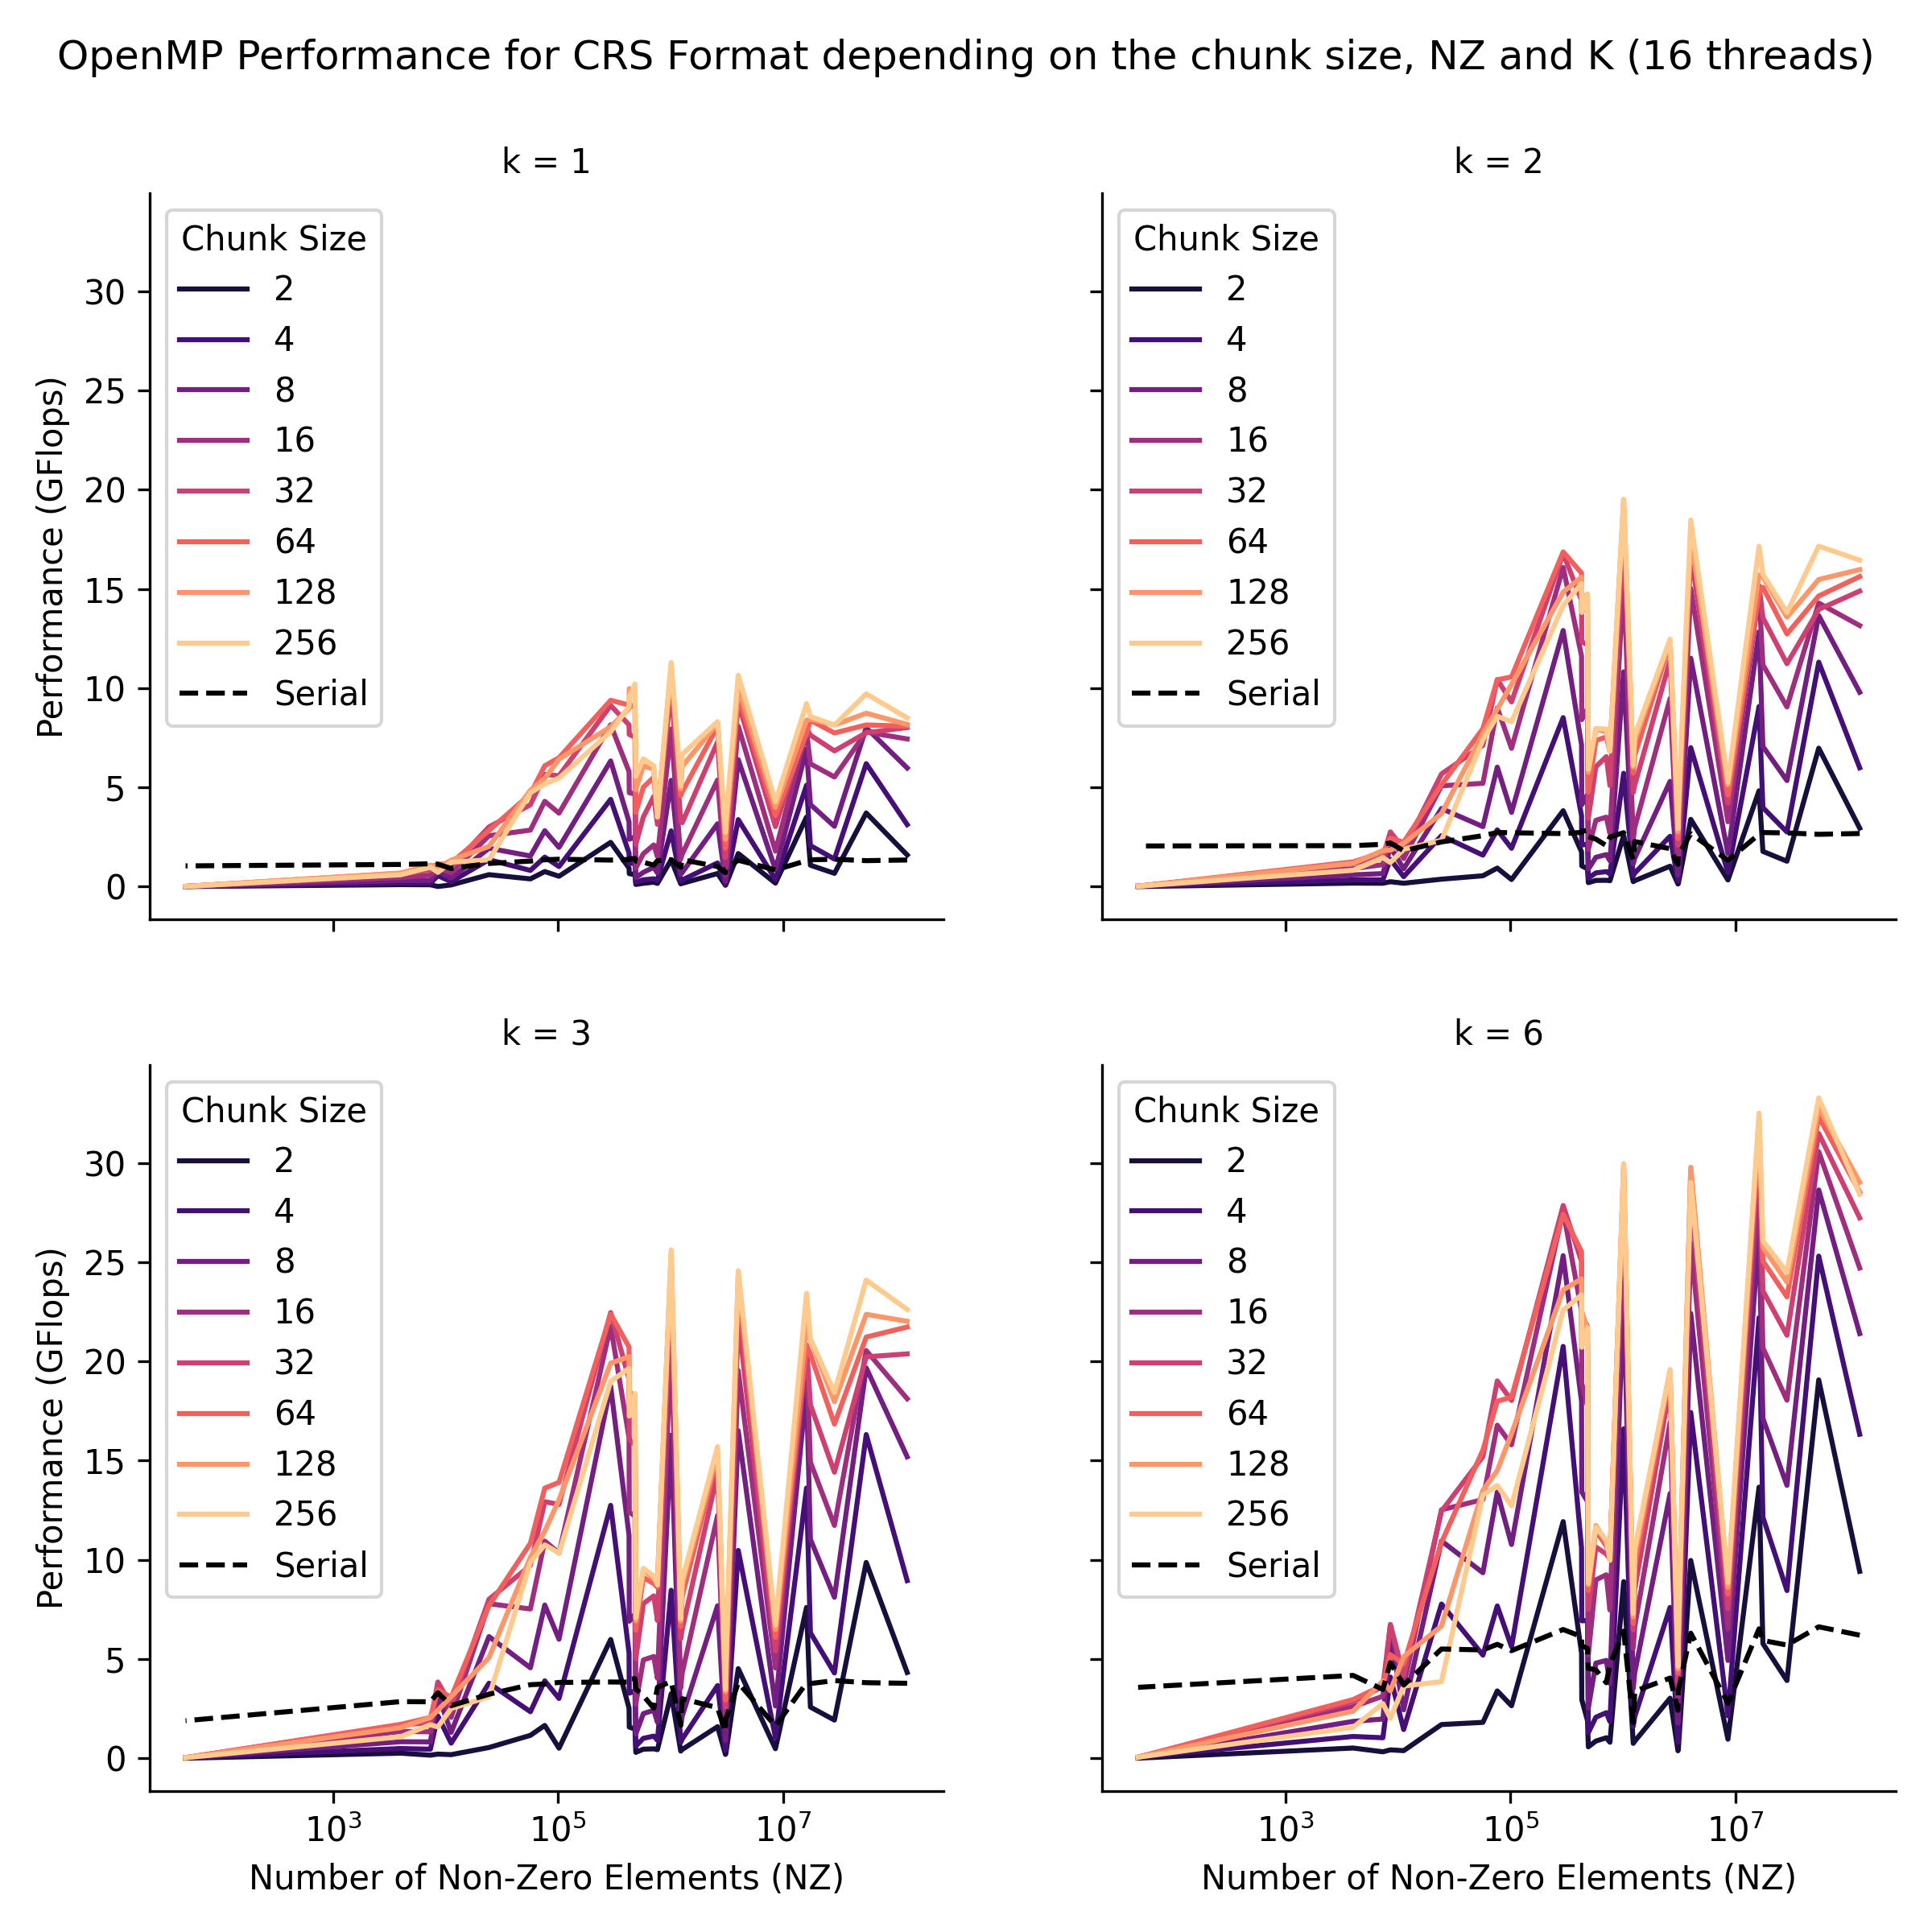
\includegraphics[width=0.75\textwidth]{../results/images/openMP_ChunkSize_CRS.png}
    \caption{OpenMP Performance for CRS Format depending on Chunk Size}
    \label{fig:openmpchunksizecrs}
\end{figure}

\begin{figure}[H]
    \centering
    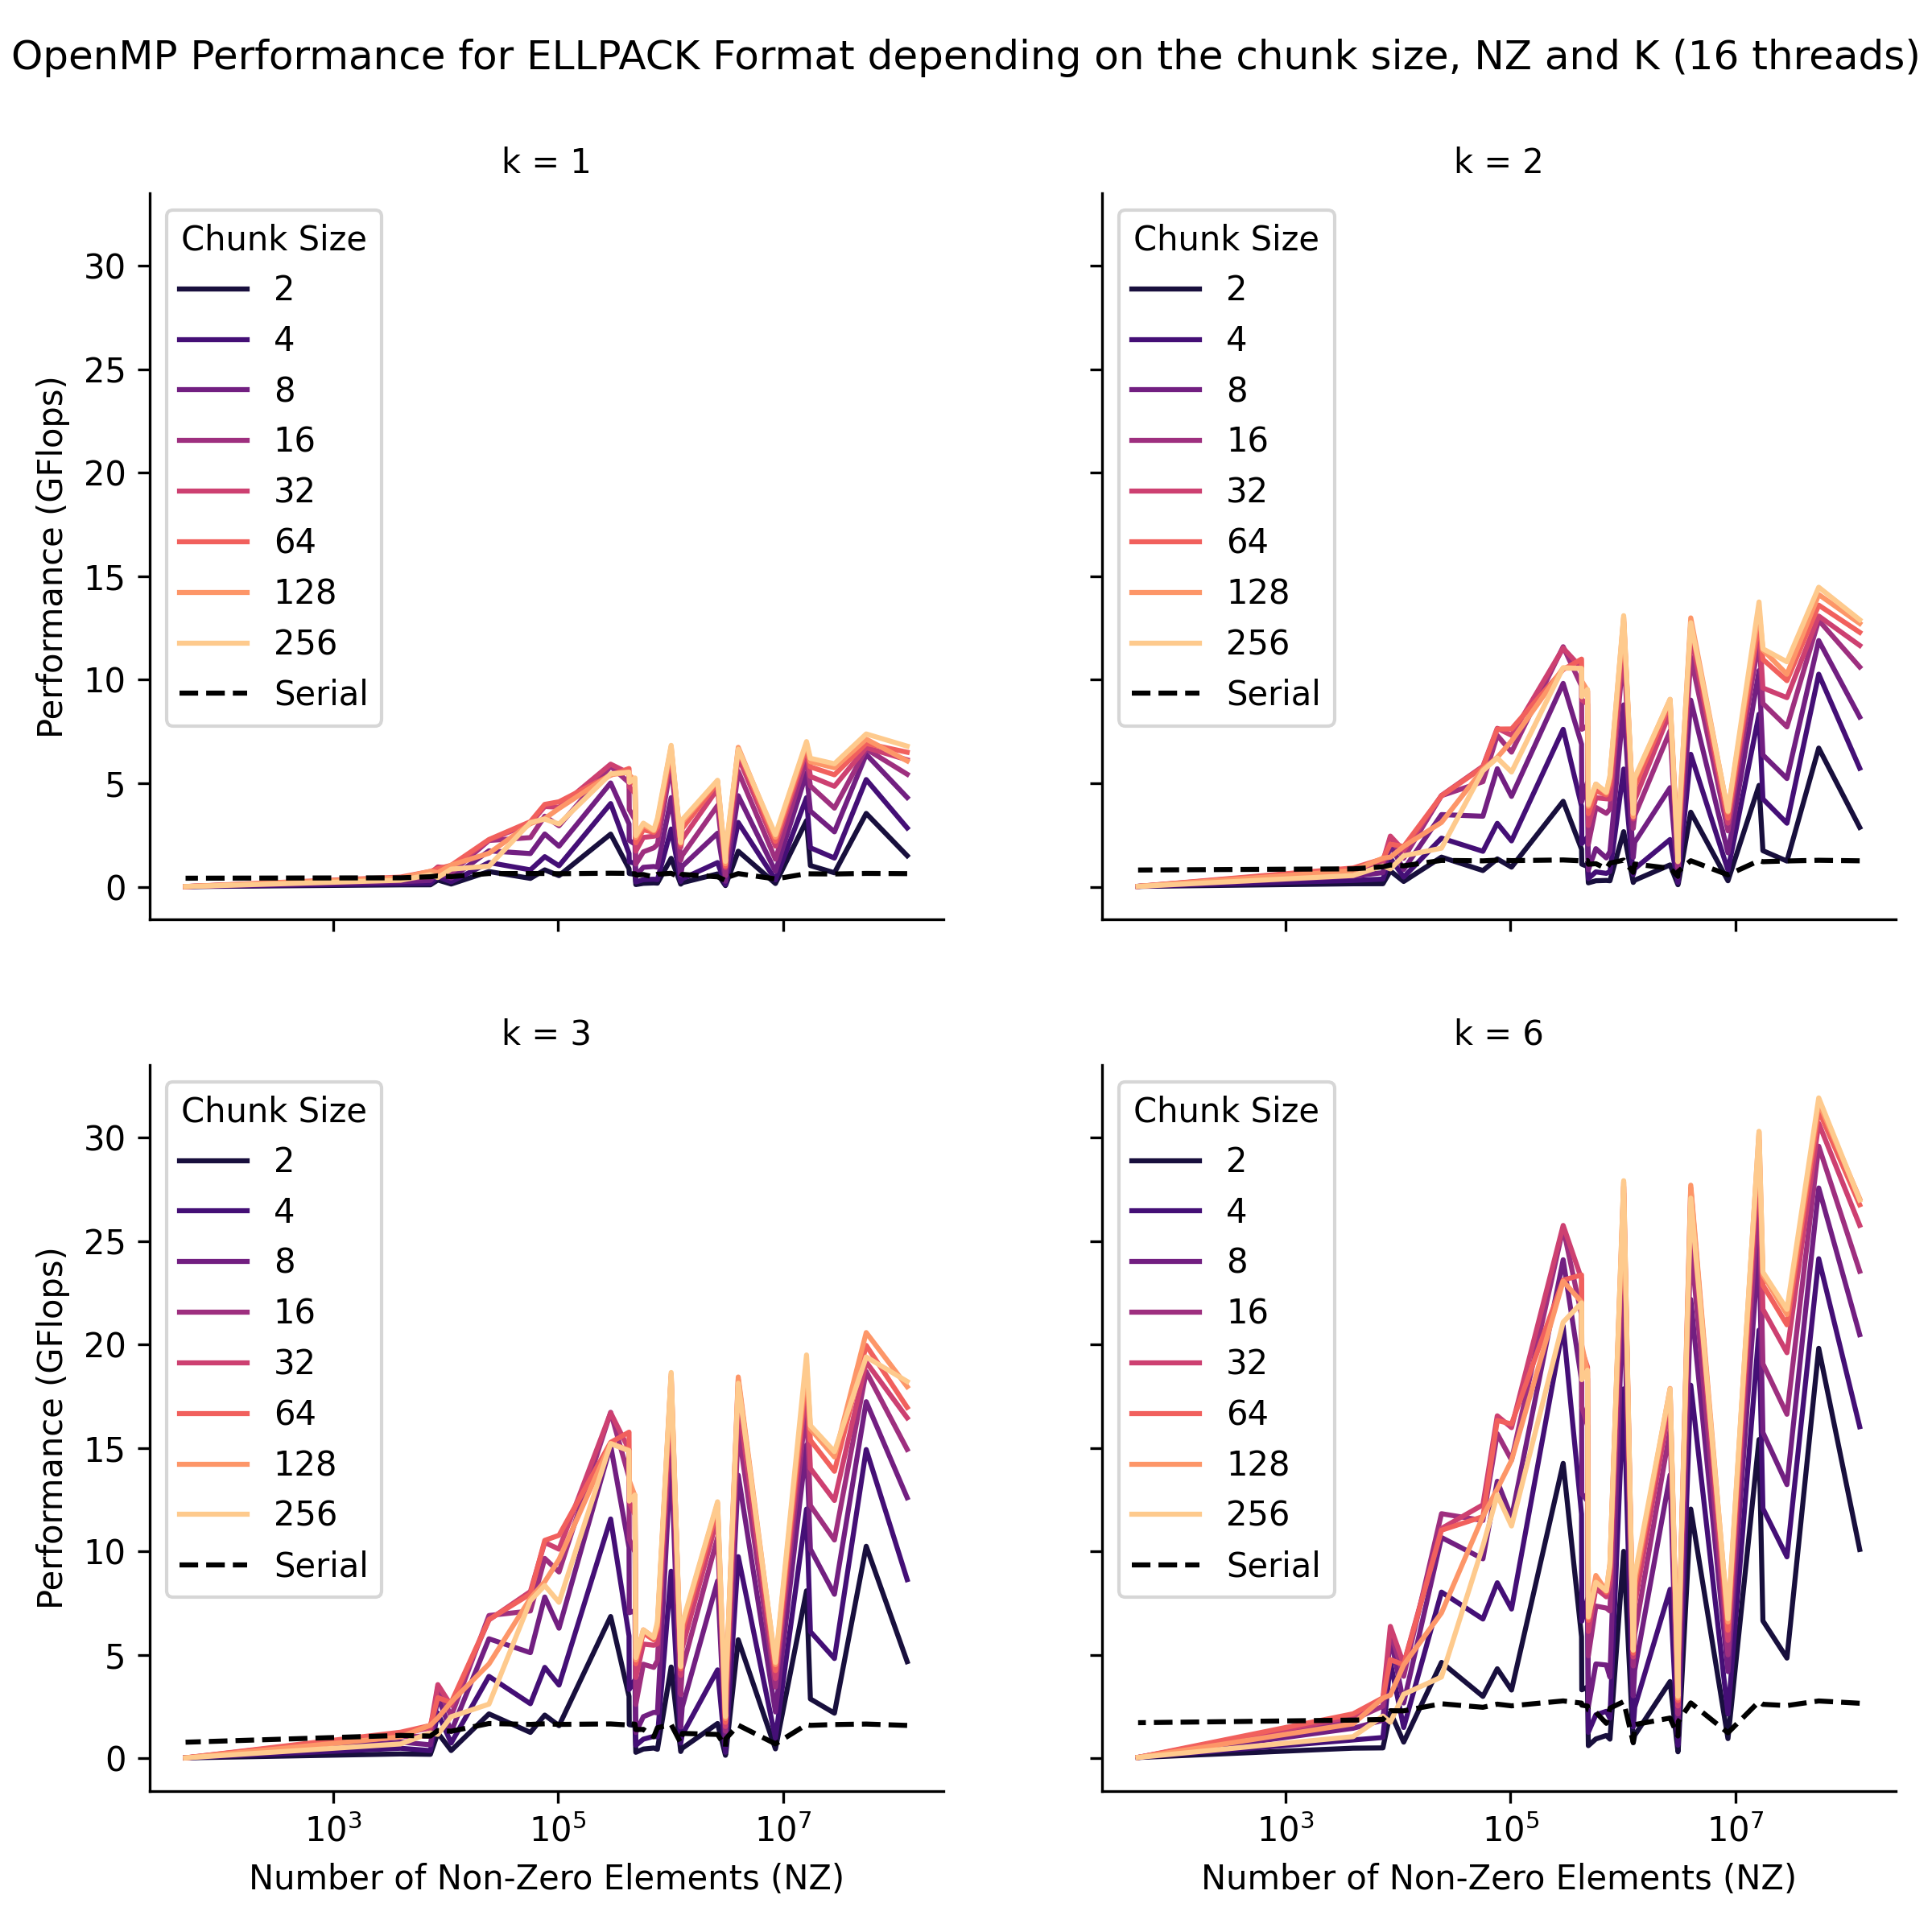
\includegraphics[width=0.75\textwidth]{../results/images/openMP_ChunkSize_ELLPACK.png}
    \caption{OpenMP Performance for ELLPACK Format depending on Chunk Size}
    \label{fig:openmpchunksizellpack}
\end{figure}

\begin{figure}[H]
    \centering
    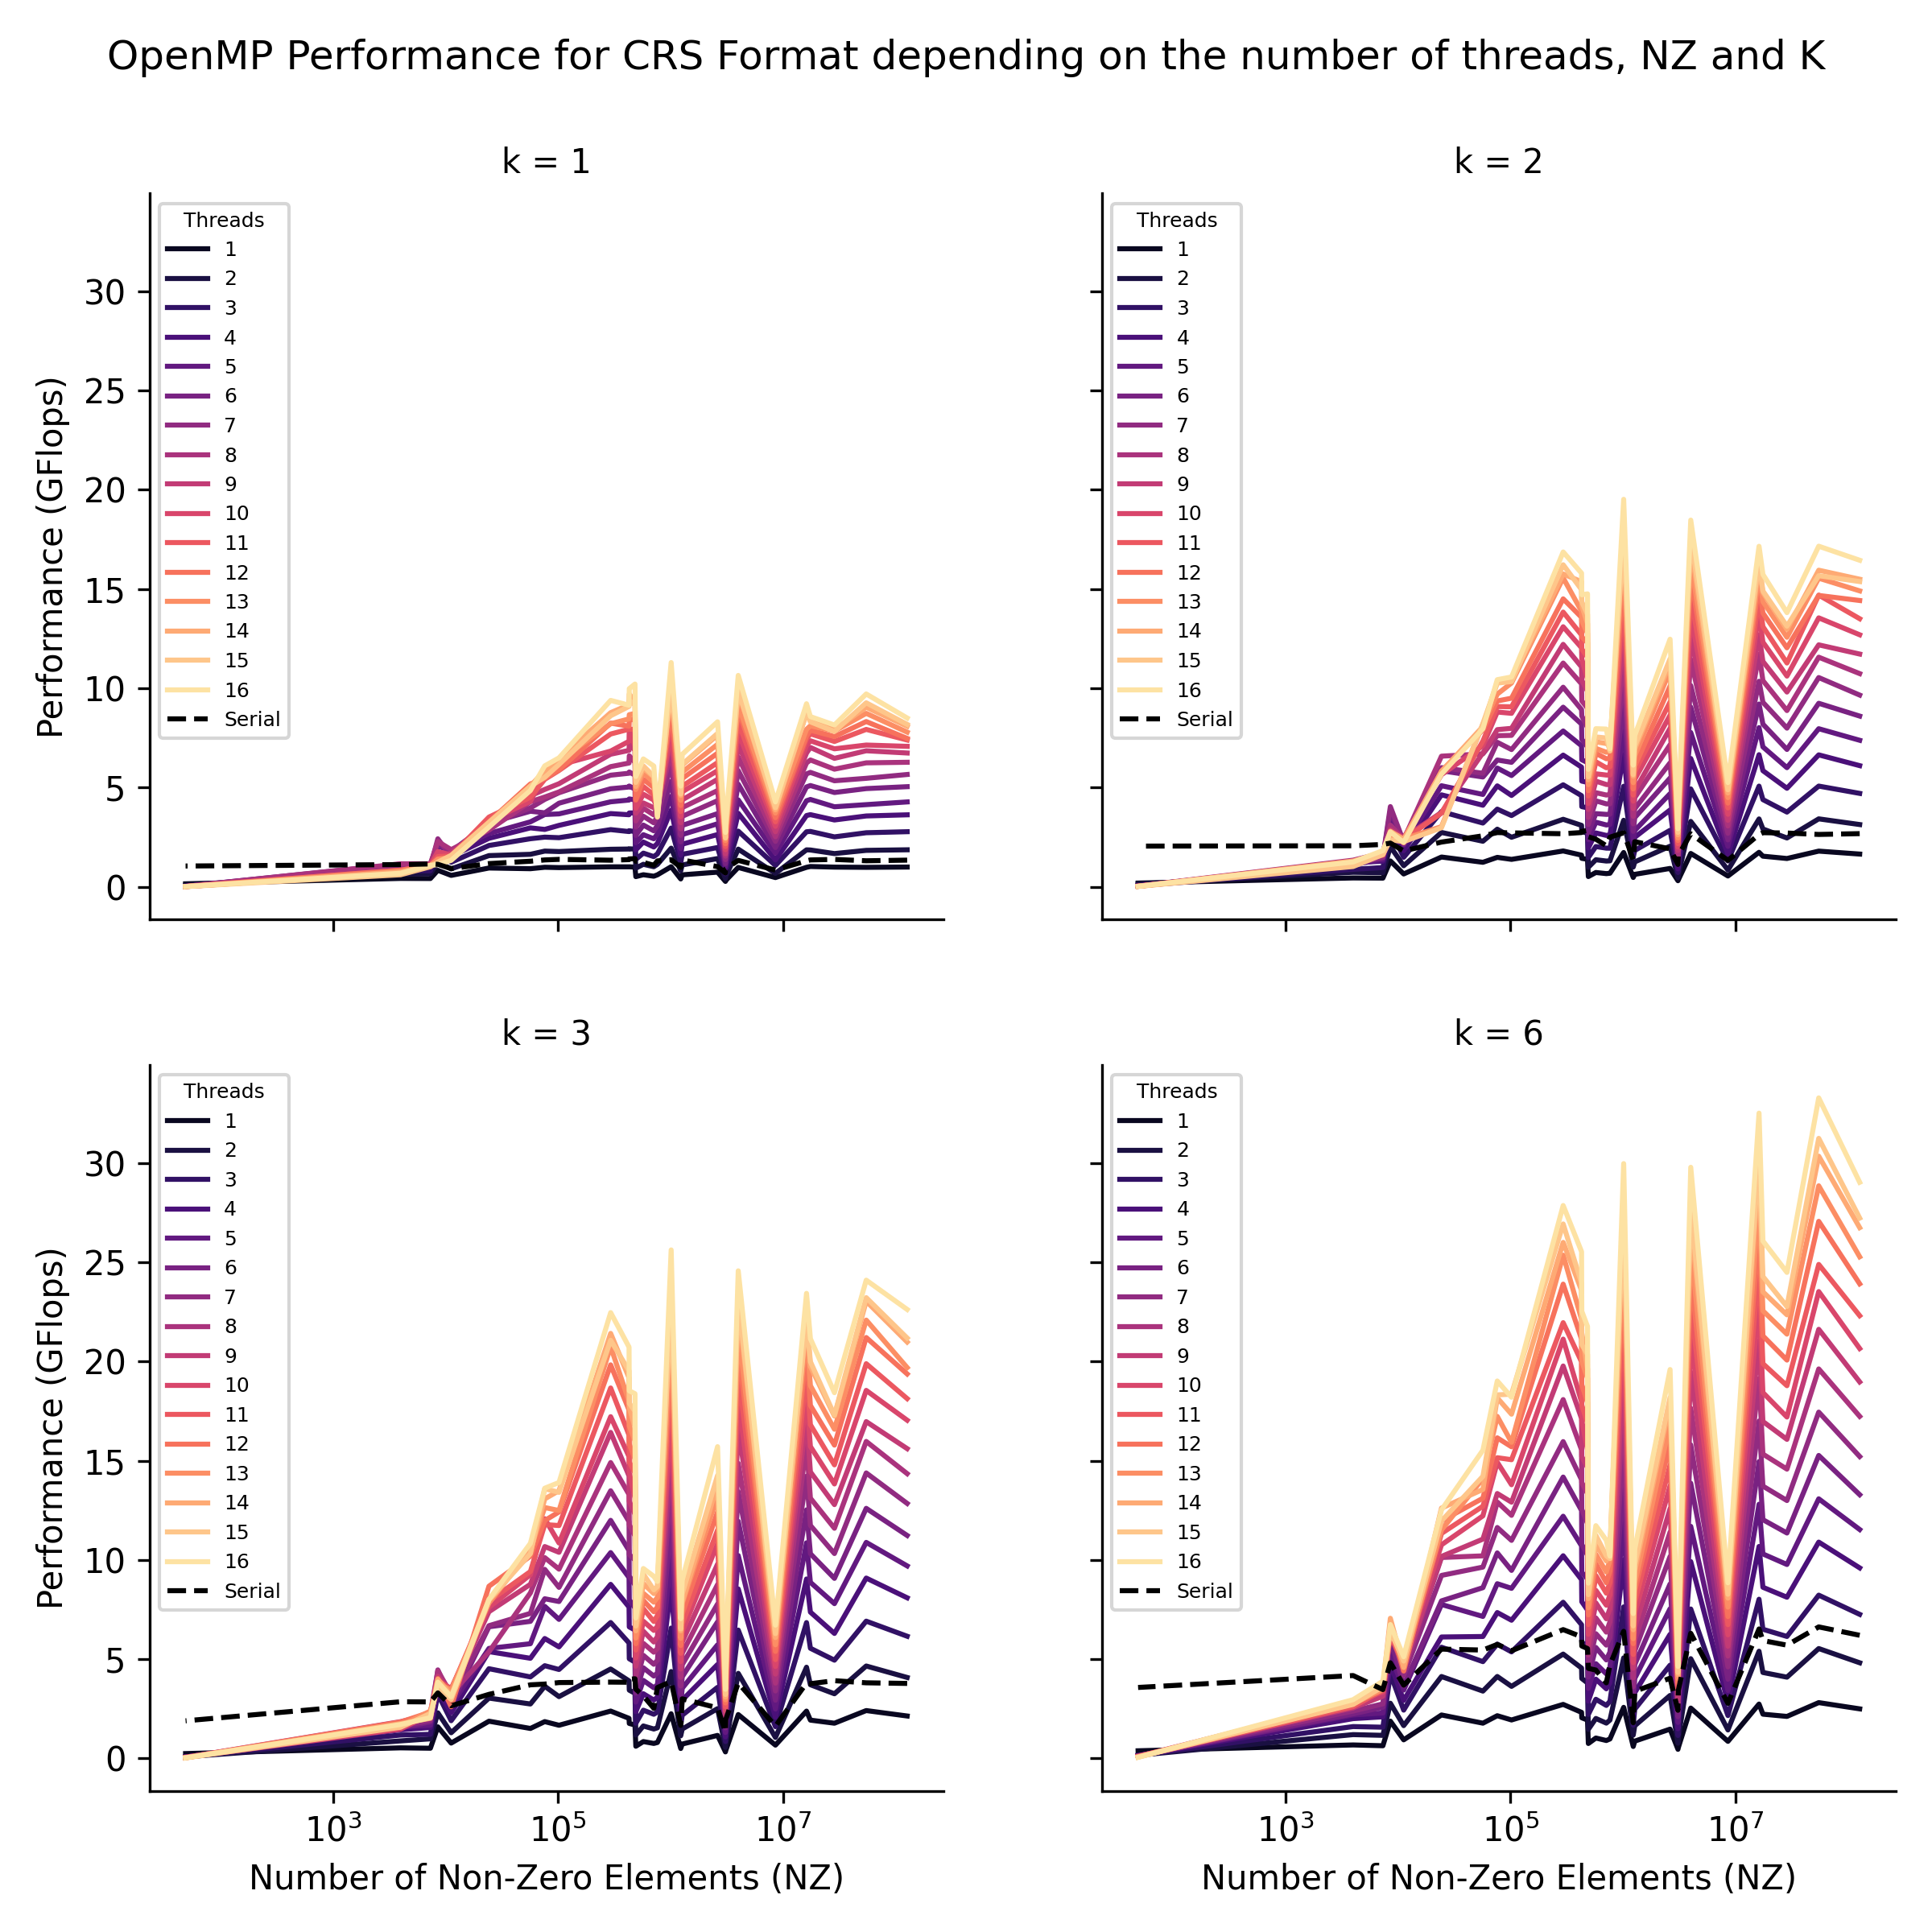
\includegraphics[width=0.75\textwidth]{../results/images/openMP_Threads_CRS.png}
    \caption{OpenMP Performance for CRS Format depending on Threads}
    \label{fig:openmpthreadscrs}
\end{figure}

\begin{figure}[H]
    \centering
    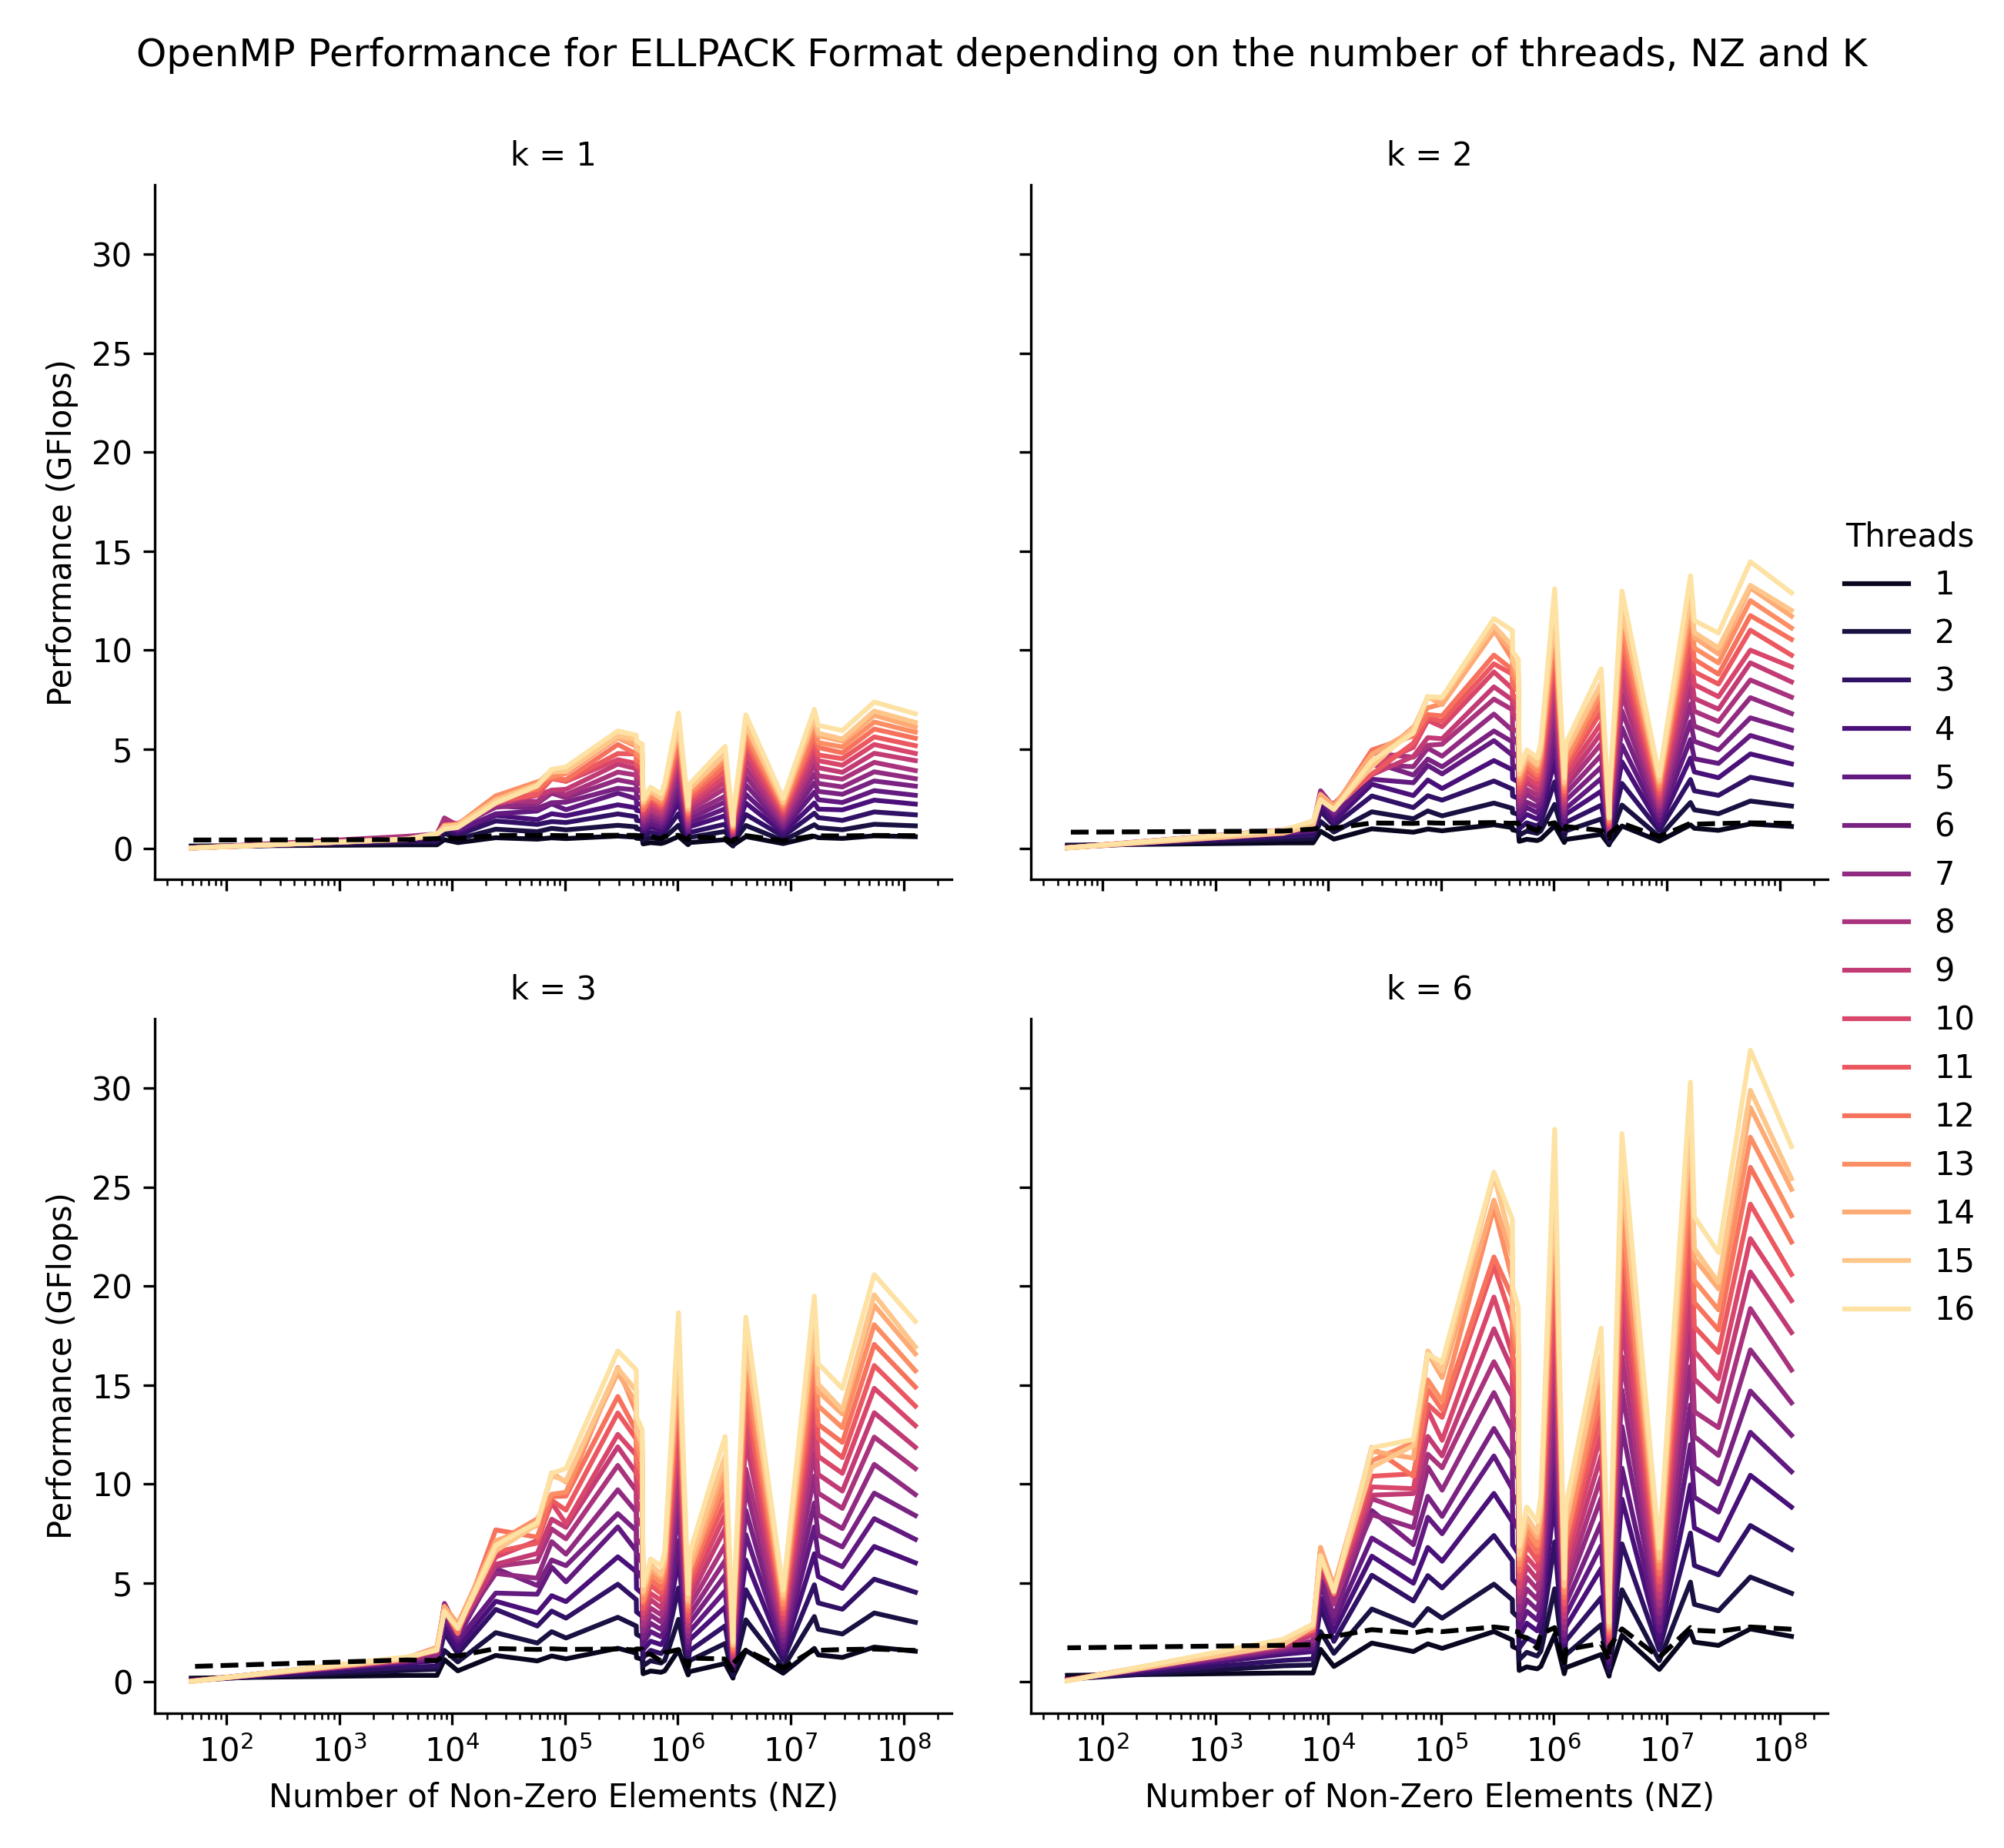
\includegraphics[width=0.75\textwidth]{../results/images/openMP_Threads_ELLPACK.png}
    \caption{OpenMP Performance for ELLPACK Format depending on Threads}
    \label{fig:openmpthreadsellpack}
\end{figure}

\newpage
\begin{figure}[H]
    \centering
    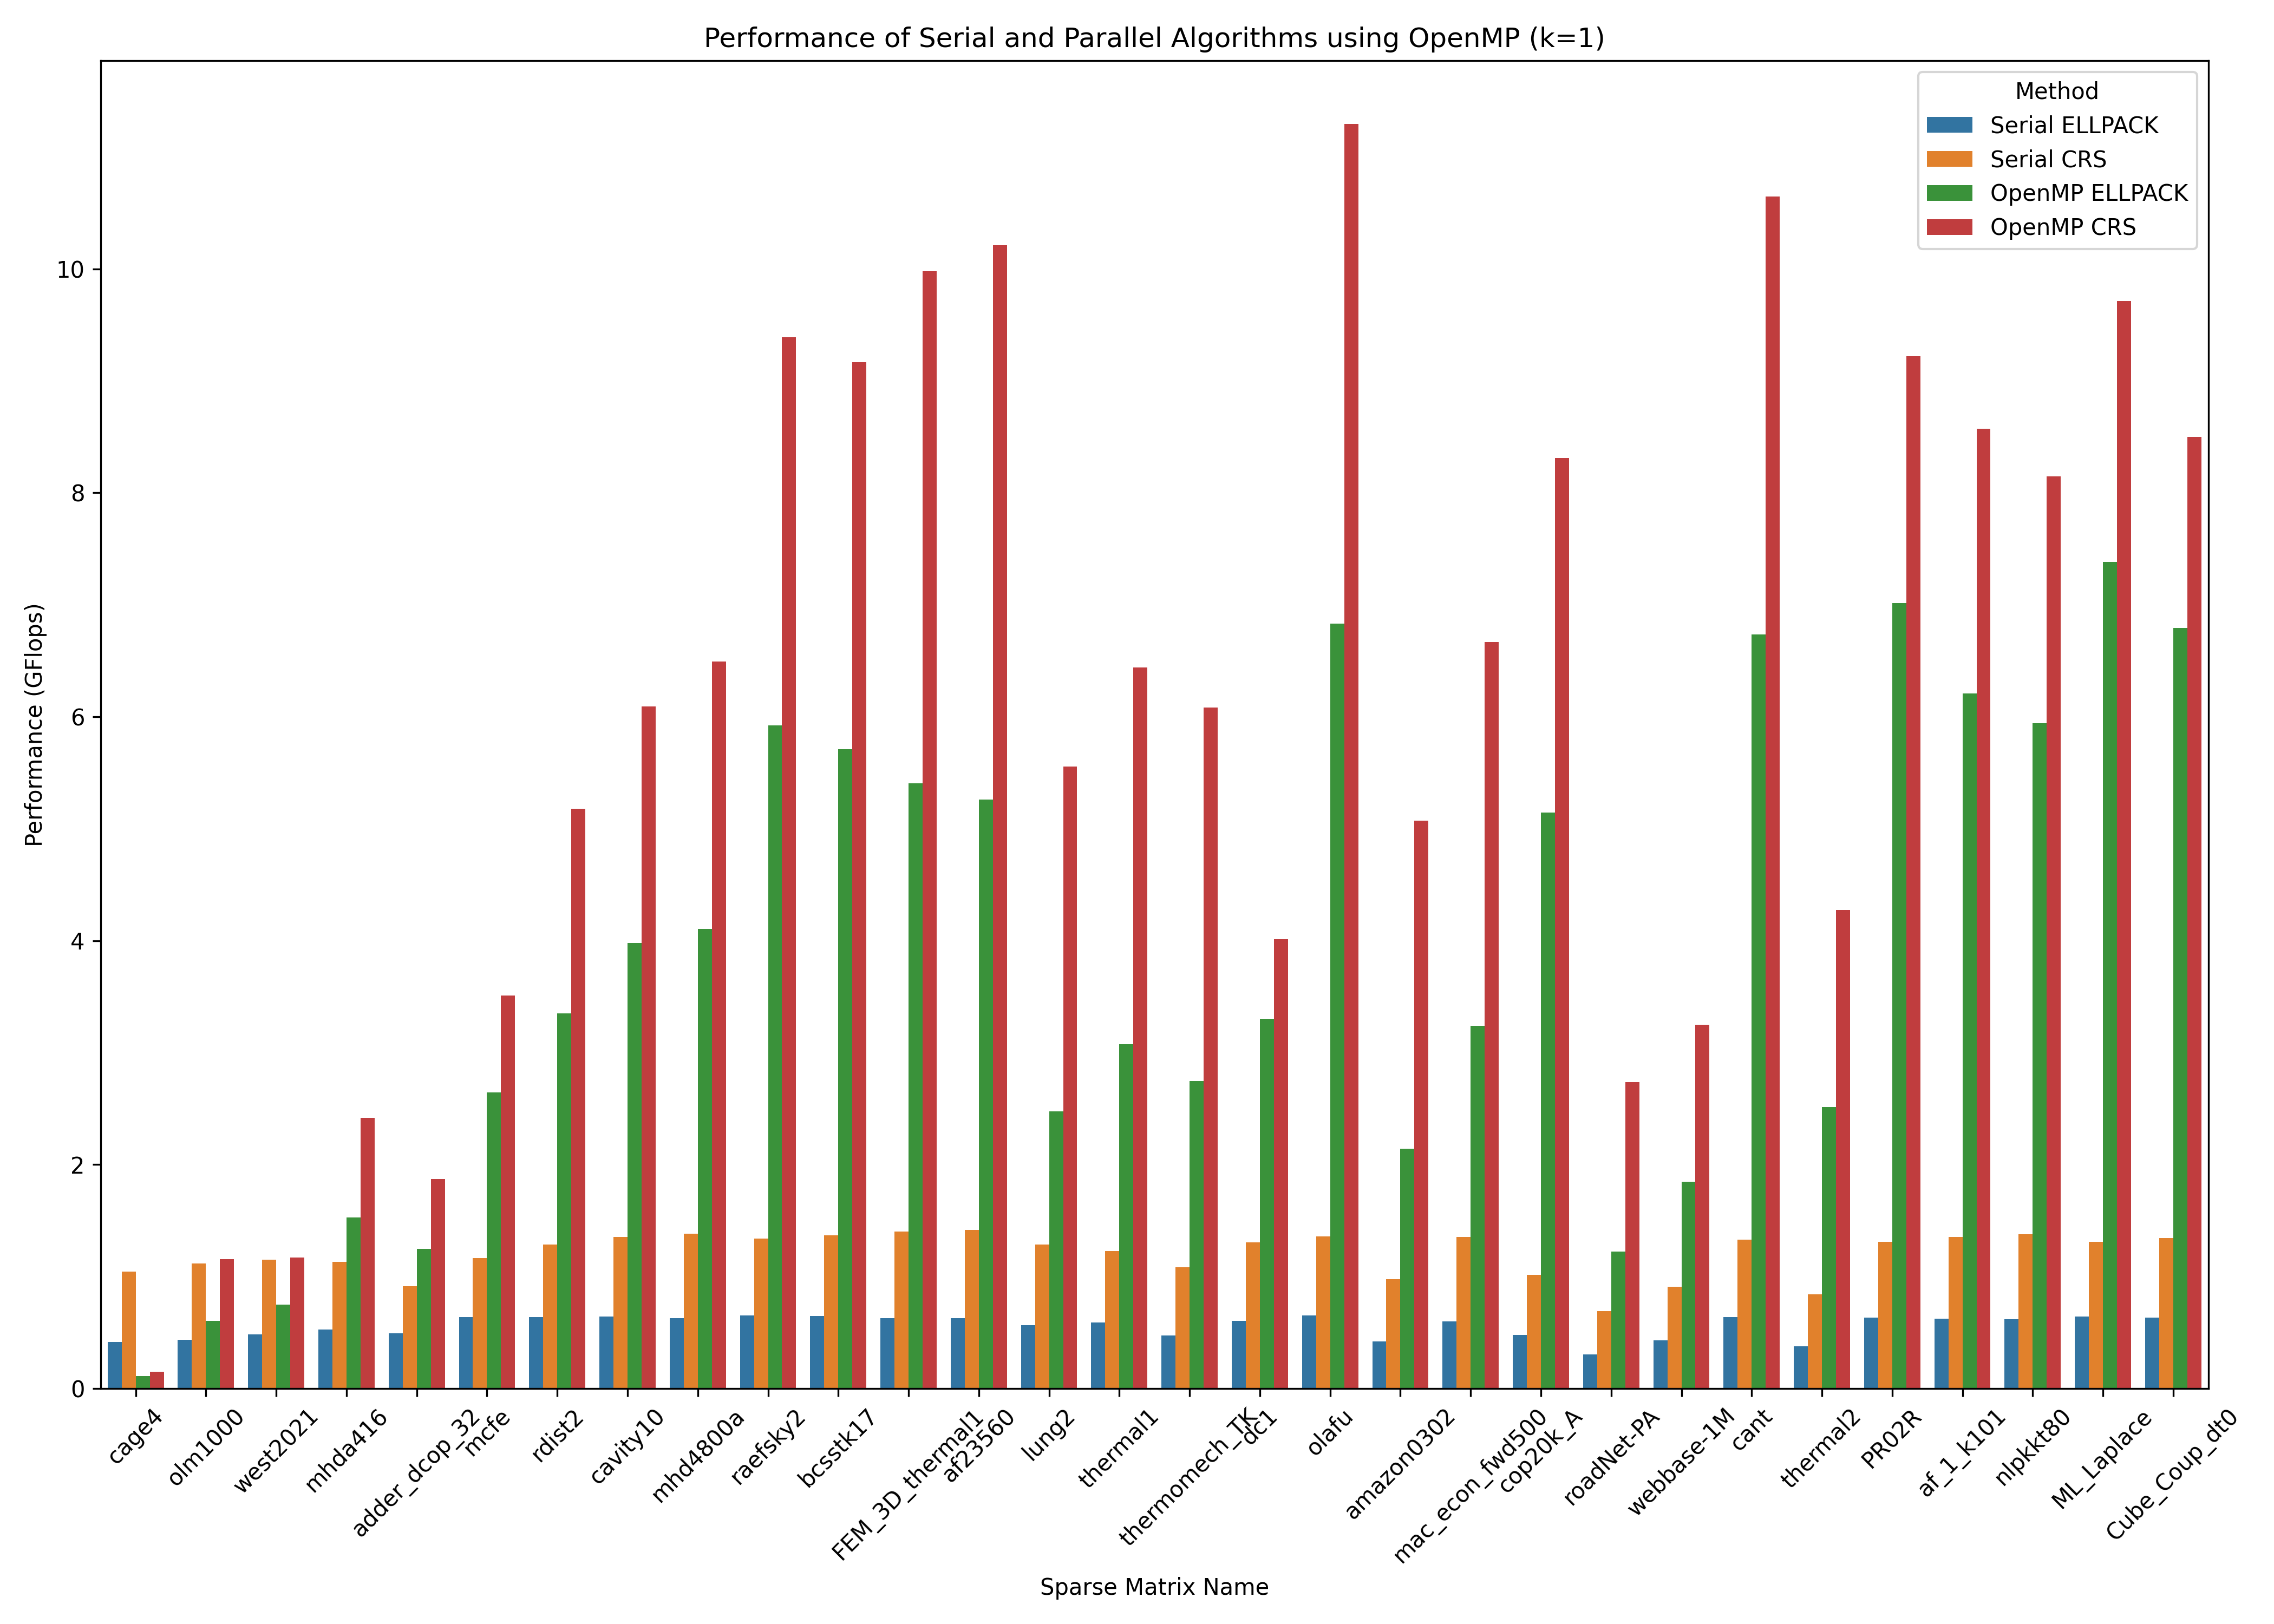
\includegraphics[width=0.9\textwidth]{../results/images/openMP_Performance_k1.png}
    \caption{Performance of Serial and Parallel Algorithms using OpenMP for $k=1$}
    \label{fig:openmp-performance-k1}
\end{figure}

\begin{figure}[H]
    \centering
    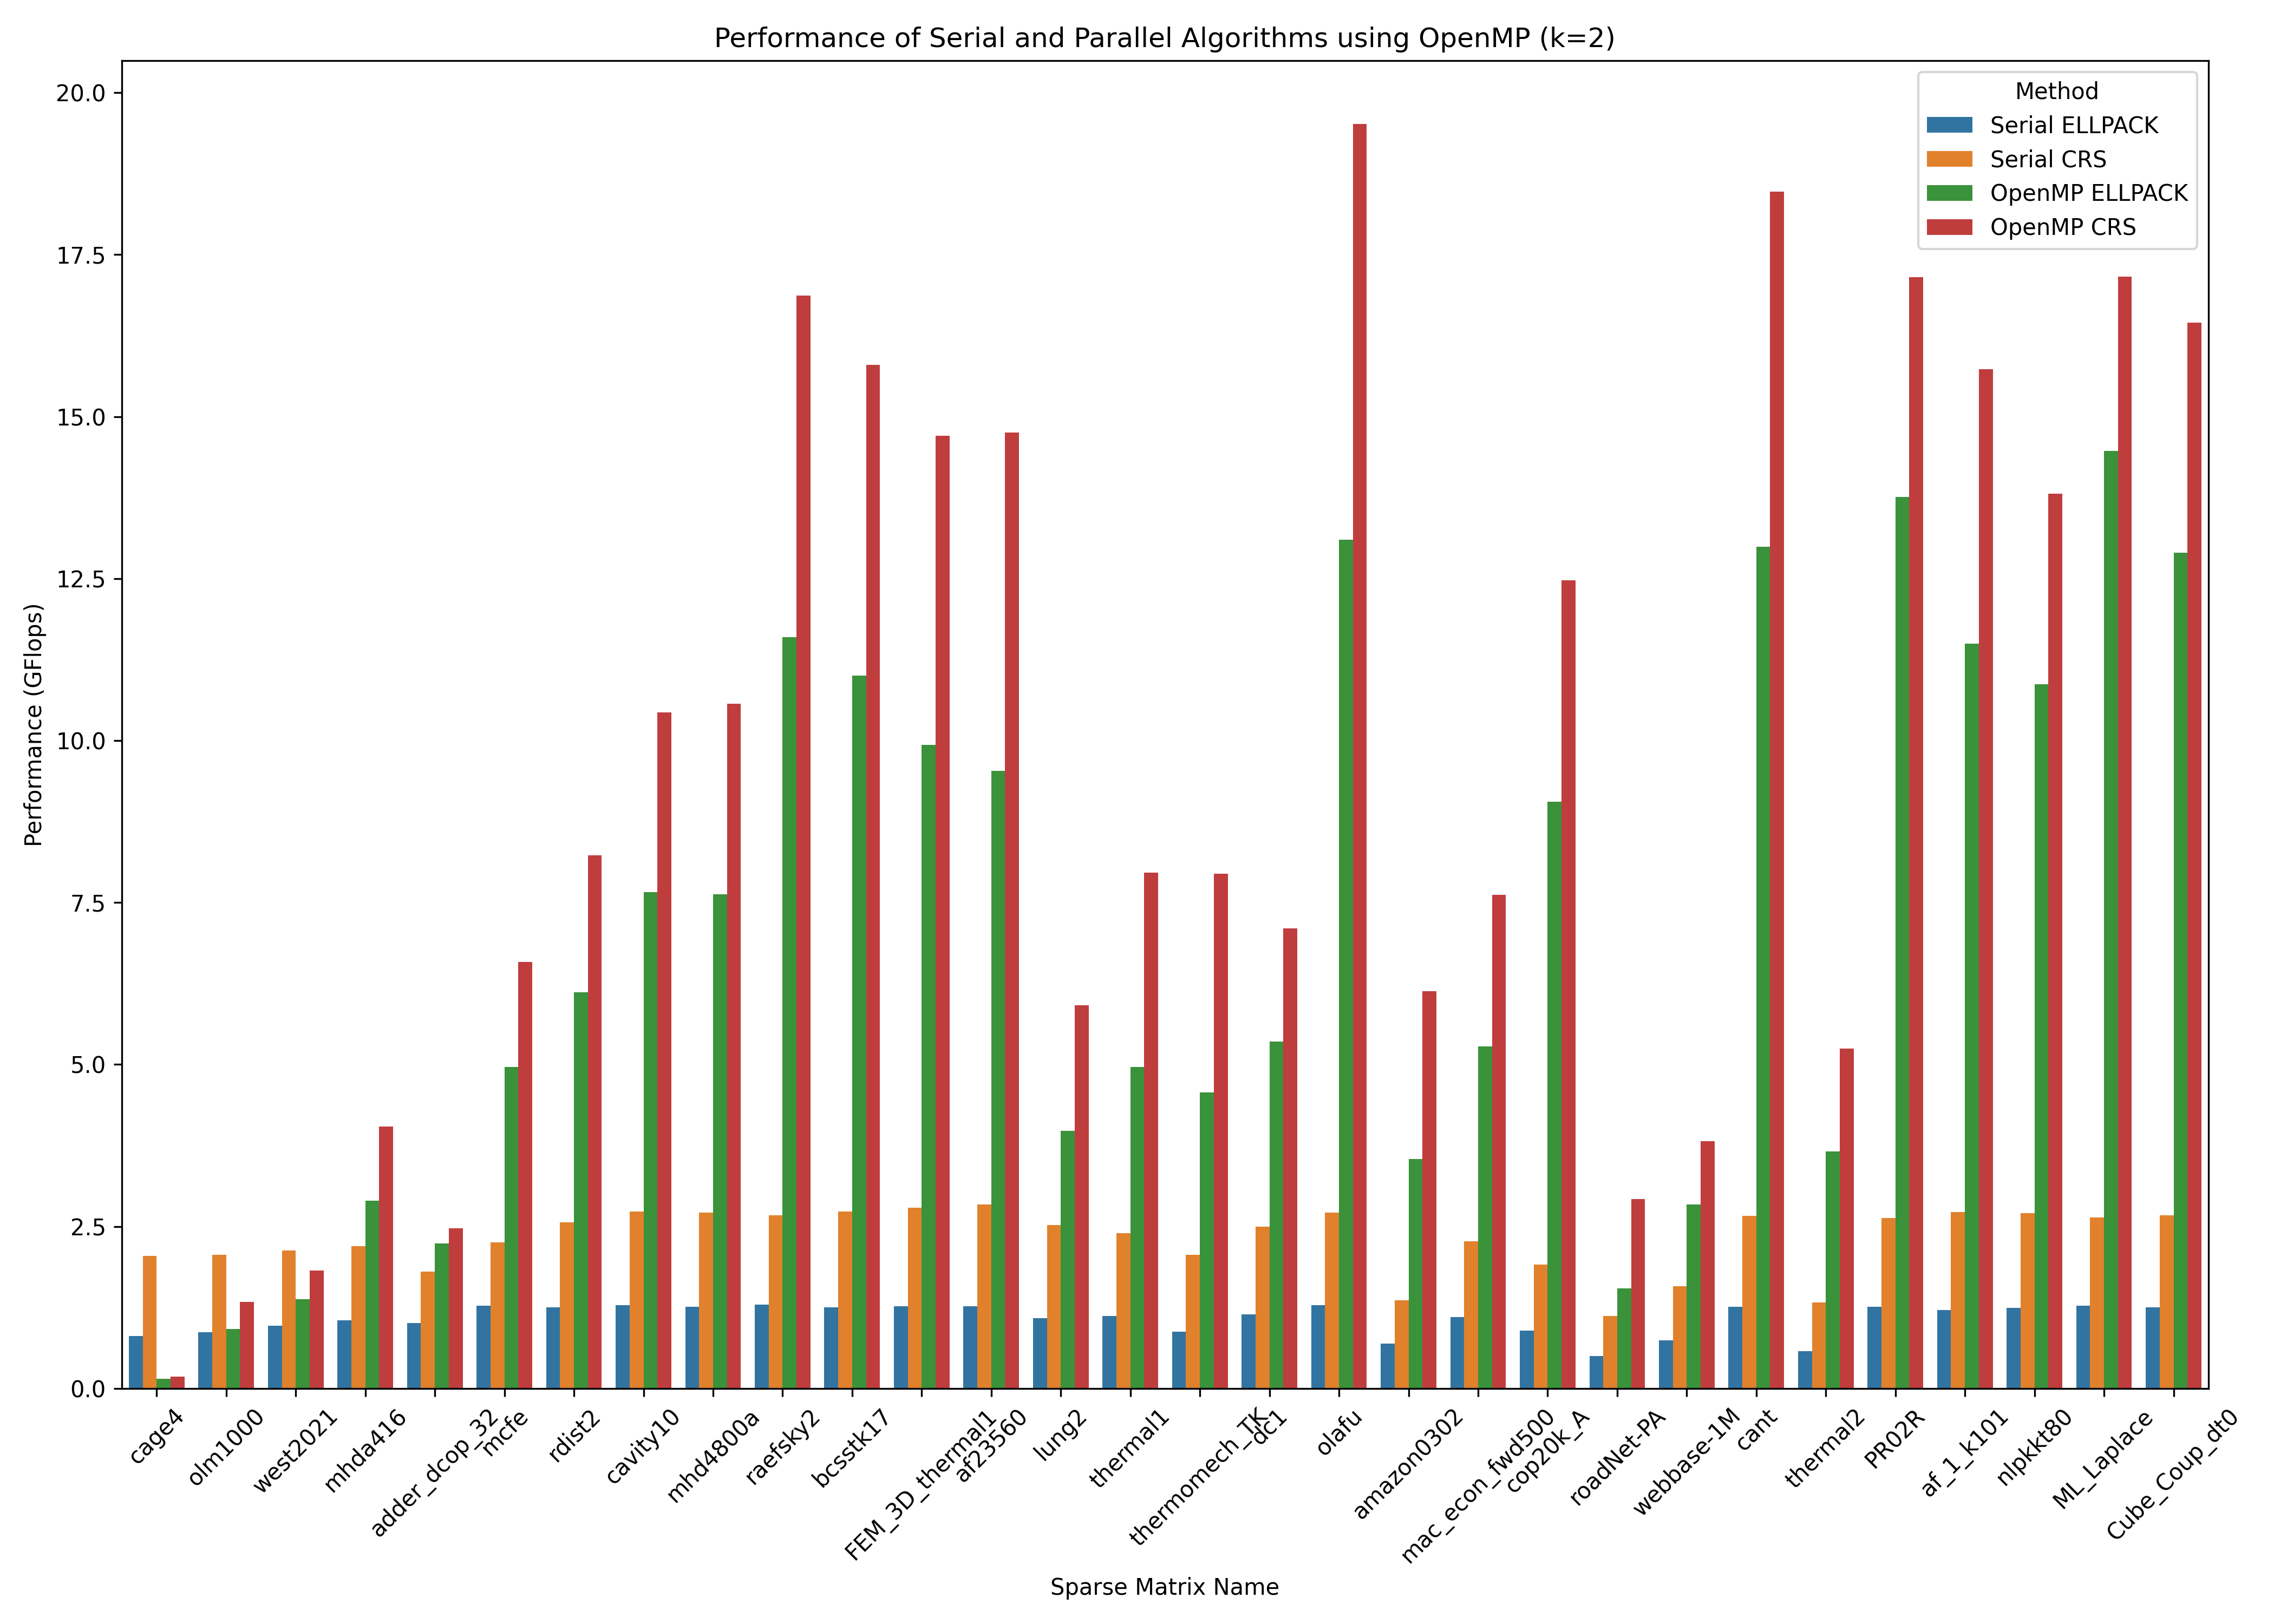
\includegraphics[width=0.9\textwidth]{../results/images/openMP_Performance_k2.png}
    \caption{Performance of Serial and Parallel Algorithms using OpenMP for $k=2$}
    \label{fig:openmp-performance-k2}
\end{figure}

\begin{figure}[H]
    \centering
    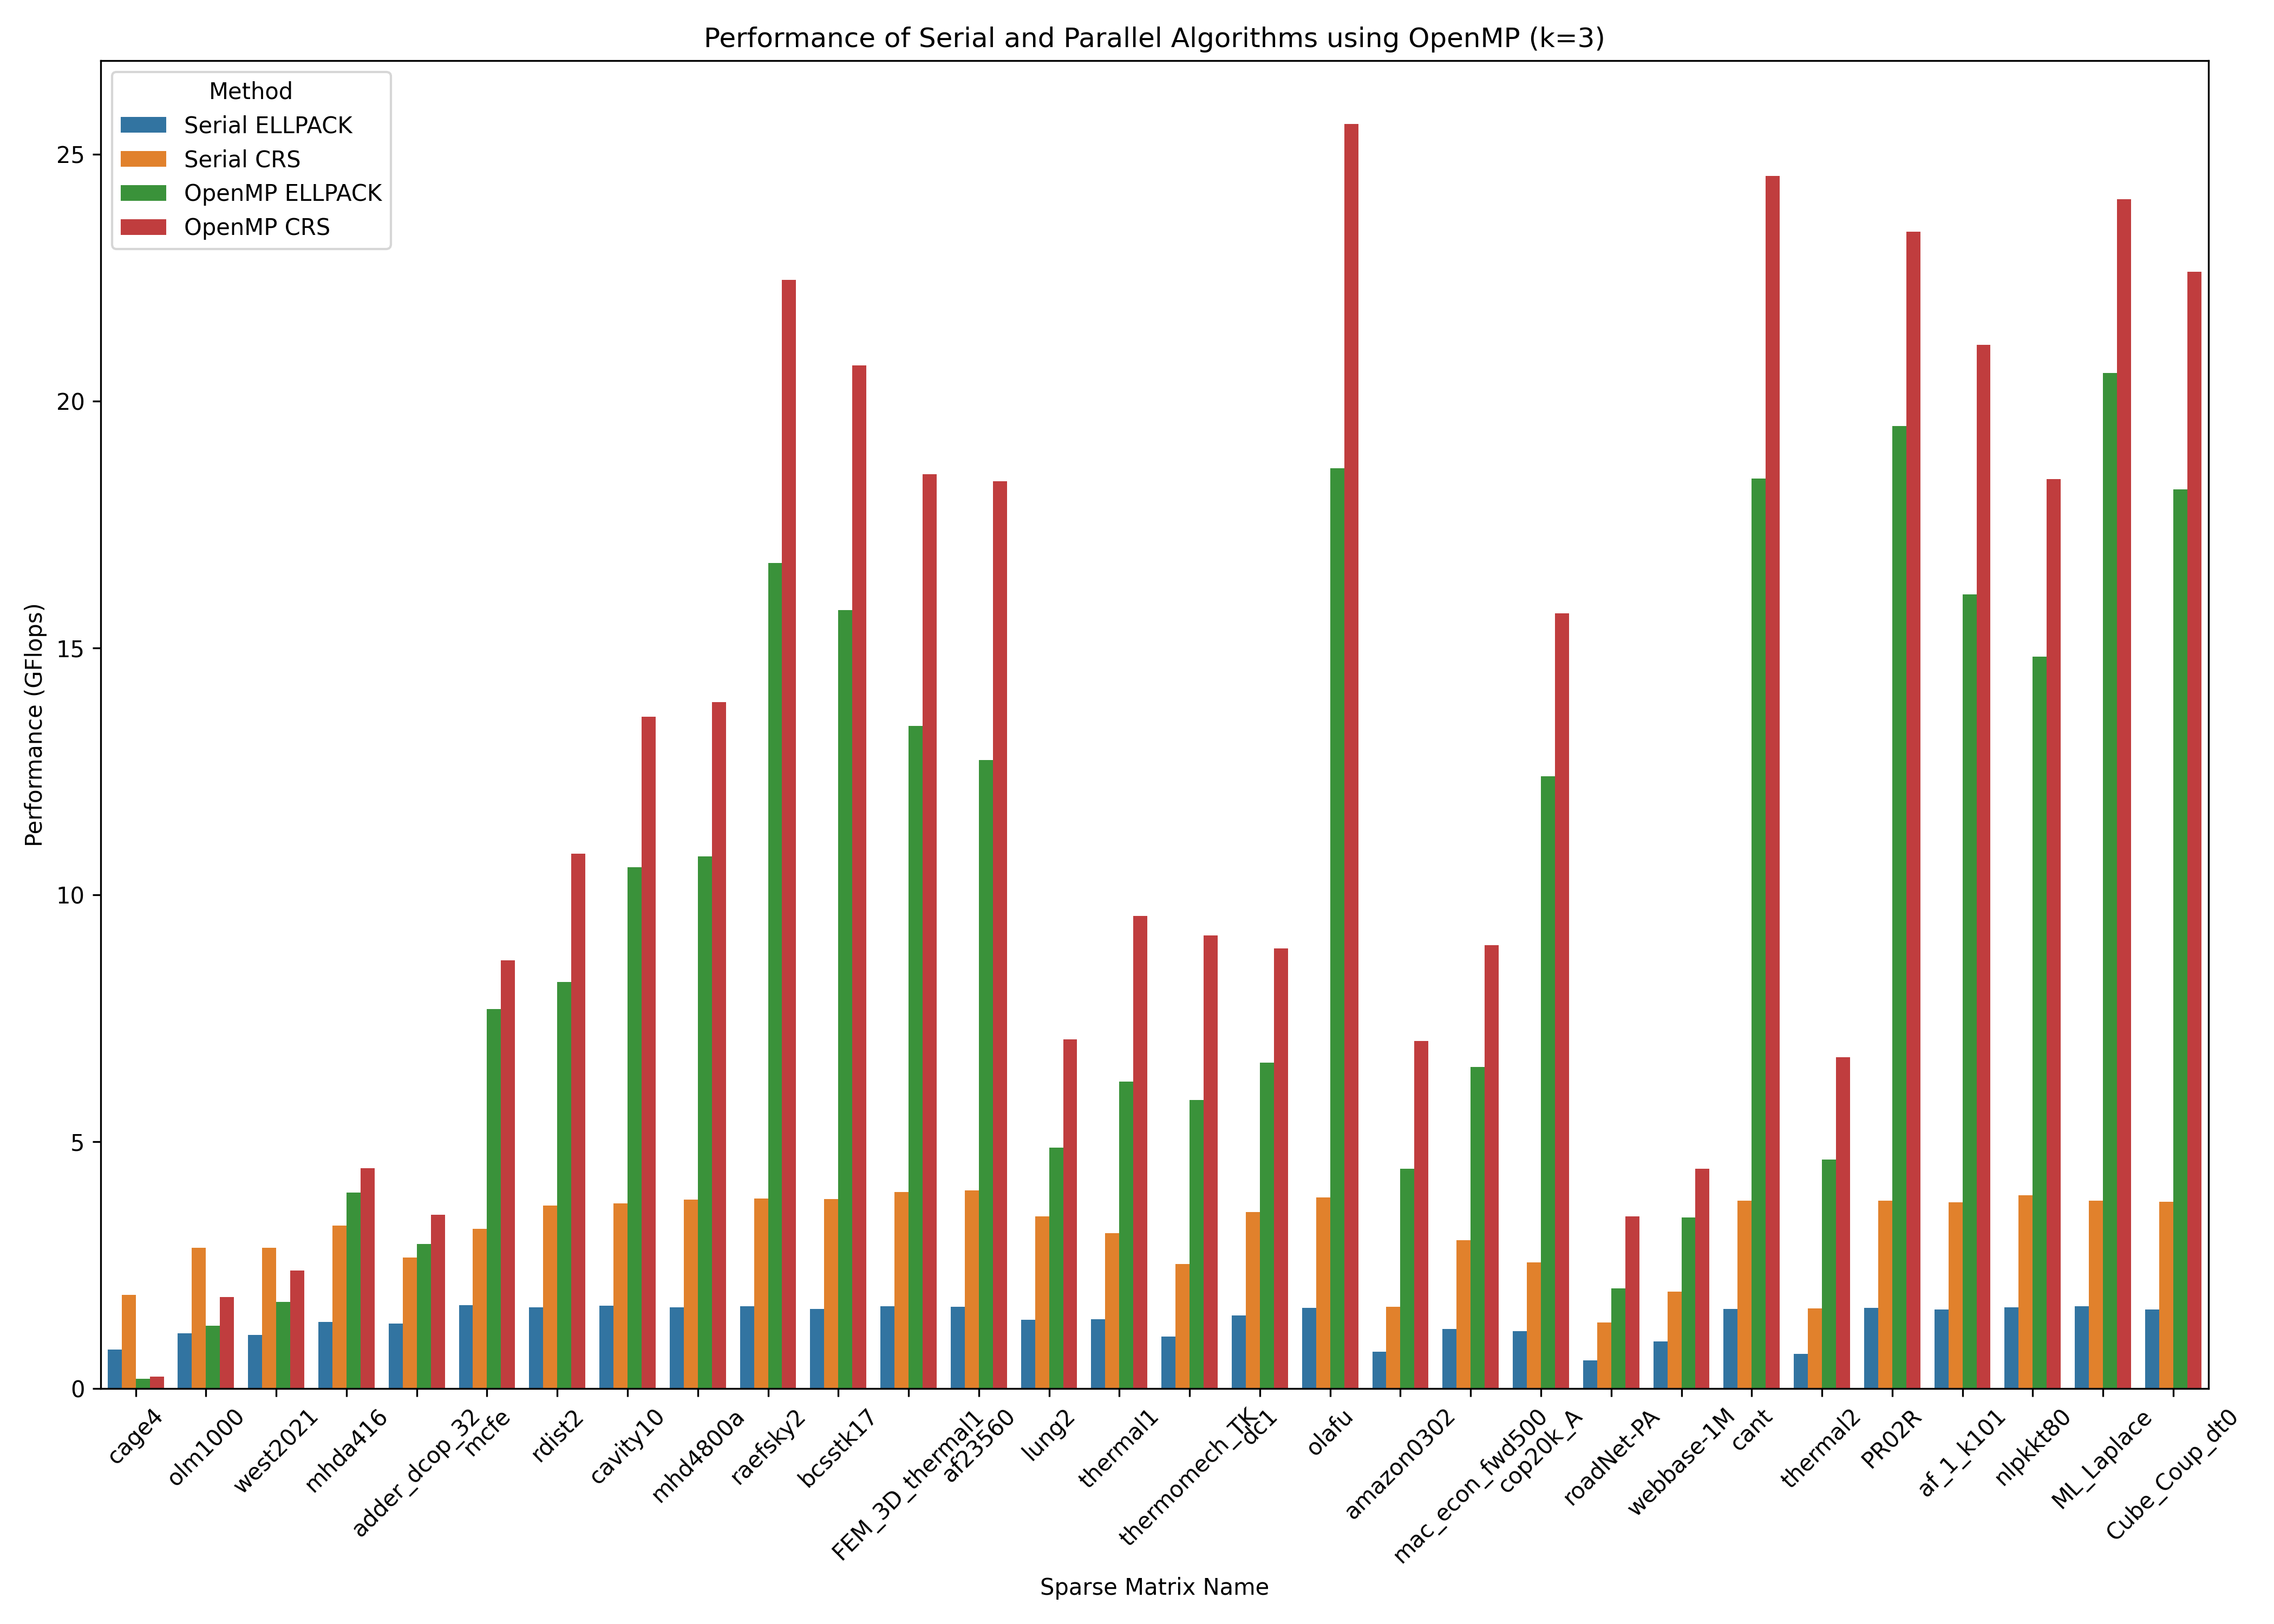
\includegraphics[width=0.9\textwidth]{../results/images/openMP_Performance_k3.png}
    \caption{Performance of Serial and Parallel Algorithms using OpenMP for $k=3$}
    \label{fig:openmp-performance-k3}
\end{figure}

\begin{figure}[H]
    \centering
    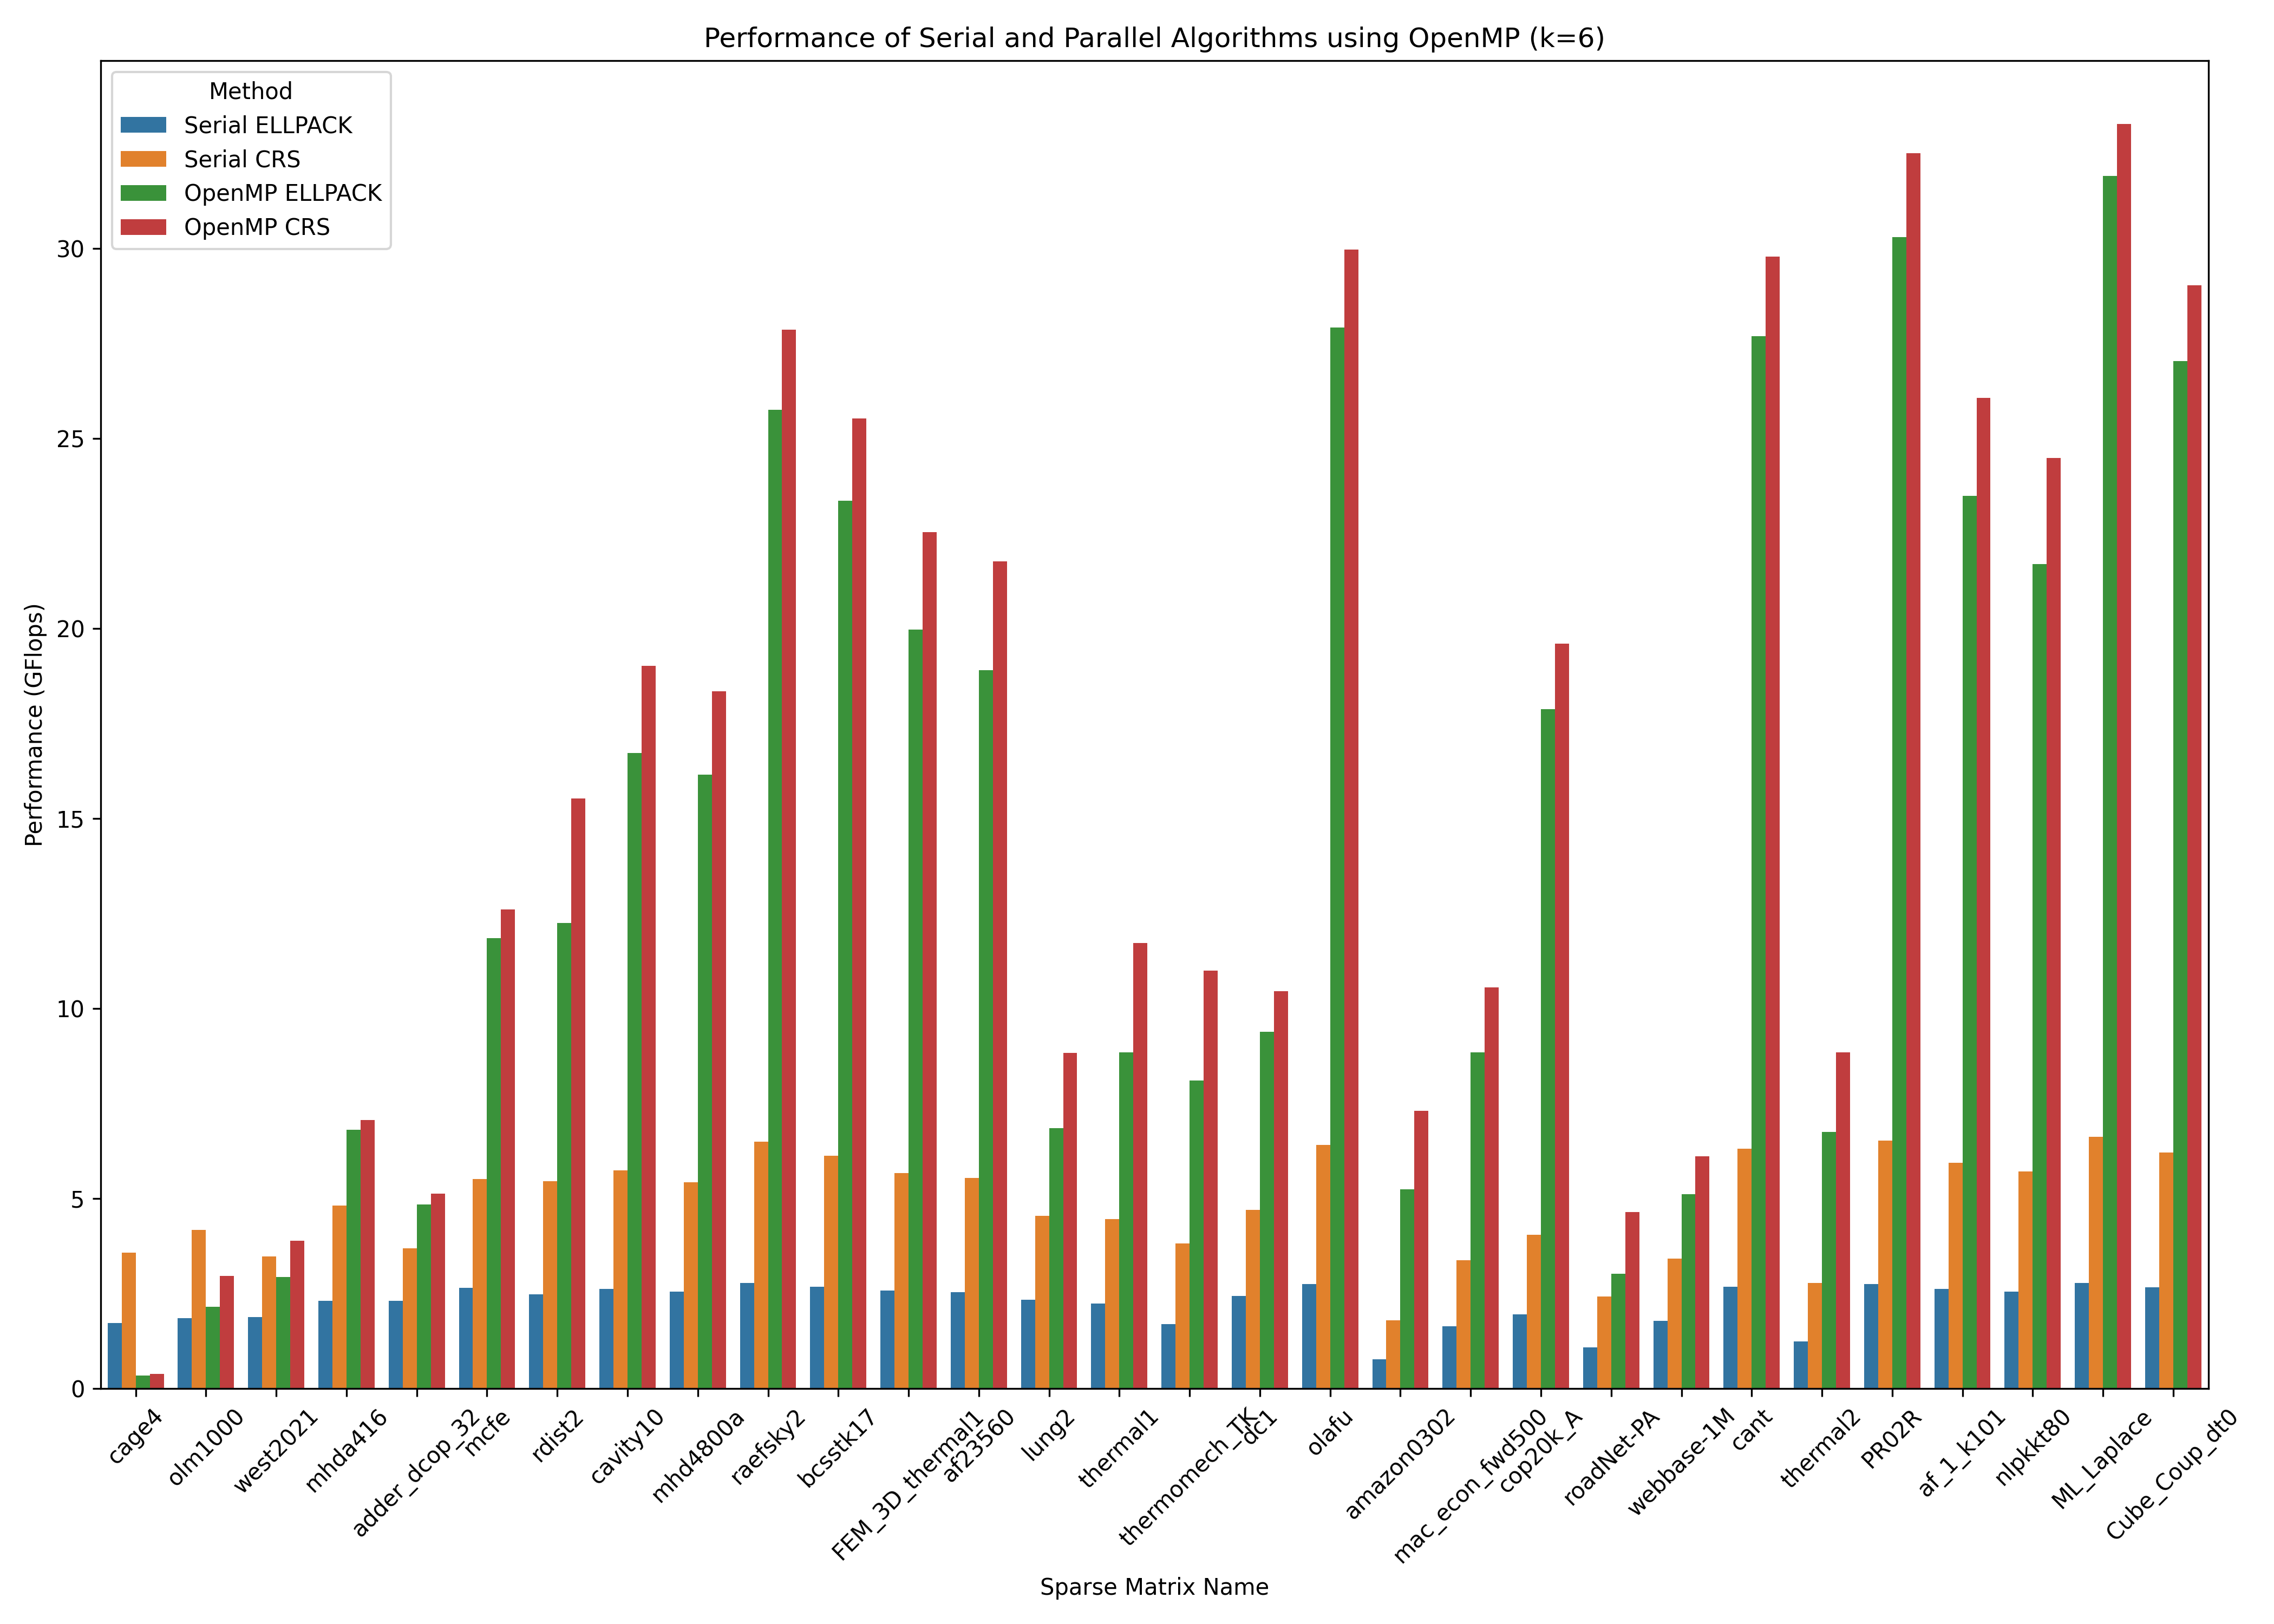
\includegraphics[width=0.9\textwidth]{../results/images/openMP_Performance_k6.png}
    \caption{Performance of Serial and Parallel Algorithms using OpenMP for $k=6$}
    \label{fig:openmp-performance-k6}
\end{figure}

\newpage
\begin{longtable}{lcccr}
    \caption{CRS vs ELLPACK avec OpenMP}                                                             \\
    \toprule
    \textbf{Matrix}   & \textbf{CRS} & \textbf{ELLPACK} & \textbf{Best Structure} & \textbf{Speedup} \\
    \midrule
    \endfirsthead
    \toprule
    \textbf{Matrix}   & \textbf{CRS} & \textbf{ELLPACK} & \textbf{Best Structure} & \textbf{Speedup} \\
    \midrule
    \endhead
    \bottomrule
    \endfoot
    Cube\_Coup\_dt0   & 29.0243      & 27.0415          & CRS                     & 4.597152         \\
    FEM\_3D\_thermal1 & 22.5277      & 19.9711          & CRS                     & 3.792766         \\
    ML\_Laplace       & 33.2766      & 31.9121          & CRS                     & 5.019799         \\
    PR02R             & 32.5086      & 30.2968          & CRS                     & 4.942094         \\
    adder\_dcop\_32   & 5.12204      & 4.83417          & CRS                     & 1.142991         \\
    af23560           & 21.7606      & 18.9078          & CRS                     & 3.748958         \\
    af\_1\_k101       & 26.067       & 23.4946          & CRS                     & 4.245709         \\
    amazon0302        & 7.29883      & 5.23835          & CRS                     & 3.113809         \\
    bcsstk17          & 25.5293      & 23.3597          & CRS                     & 4.080255         \\
    cage4             & 0.385164     & 0.334653         & CRS                     & 0.441890         \\
    cant              & 29.7794      & 27.6956          & CRS                     & 4.638745         \\
    cavity10          & 19.0148      & 16.7258          & CRS                     & 3.152232         \\
    cop20k\_A         & 19.5918      & 17.8729          & CRS                     & 4.105772         \\
    dc1               & 10.4524      & 9.39085          & CRS                     & 2.230150         \\
    lung2             & 8.832        & 6.85328          & CRS                     & 1.905592         \\
    mac\_econ\_fwd500 & 10.5515      & 8.84879          & CRS                     & 2.863691         \\
    mcfe              & 12.6097      & 11.8456          & CRS                     & 2.077682         \\
    mhd4800a          & 18.3501      & 16.1582          & CRS                     & 3.352021         \\
    mhda416           & 7.06099      & 6.80262          & CRS                     & 1.278130         \\
    nlpkkt80          & 24.4853      & 21.694           & CRS                     & 4.127566         \\
    olafu             & 29.966       & 27.9111          & CRS                     & 4.623662         \\
    olm1000           & 2.95895      & 2.1558           & CRS                     & 0.619634         \\
    raefsky2          & 27.8548      & 25.7504          & CRS                     & 4.248730         \\
    rdist2            & 15.5283      & 12.2527          & CRS                     & 2.694487         \\
    roadNet-PA        & 4.63584      & 3.01227          & CRS                     & 1.703601         \\
    thermal1          & 11.7254      & 8.83925          & CRS                     & 2.549122         \\
    thermal2          & 8.84723      & 6.75174          & CRS                     & 2.758931         \\
    thermomech\_TK    & 10.9908      & 8.10205          & CRS                     & 3.088284         \\
    webbase-1M        & 6.11469      & 5.10783          & CRS                     & 1.630393         \\
    west2021          & 3.89256      & 2.92762          & CRS                     & 0.930255         \\                                                                               \\
\end{longtable}

\newpage
\begin{figure}[H]
    \centering
    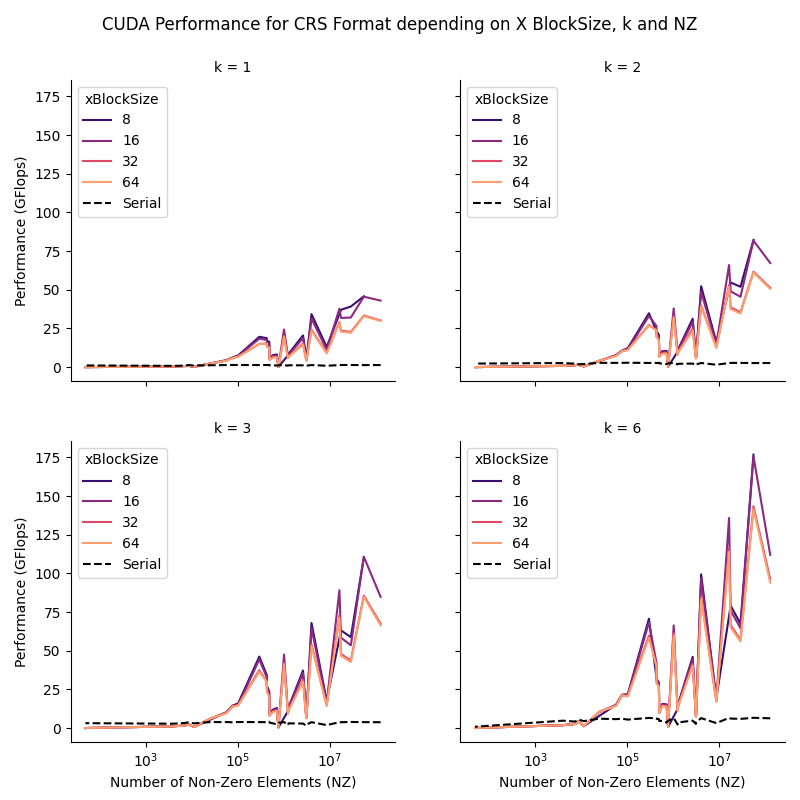
\includegraphics[width=0.75\textwidth]{../results/images/CUDA_xBlockSize_CRS.png}
    \caption{CUDA Performance for CRS Format depending on X BlockSize}
    \label{fig:cudaxblocksizecrs}
\end{figure}

\begin{figure}[H]
    \centering
    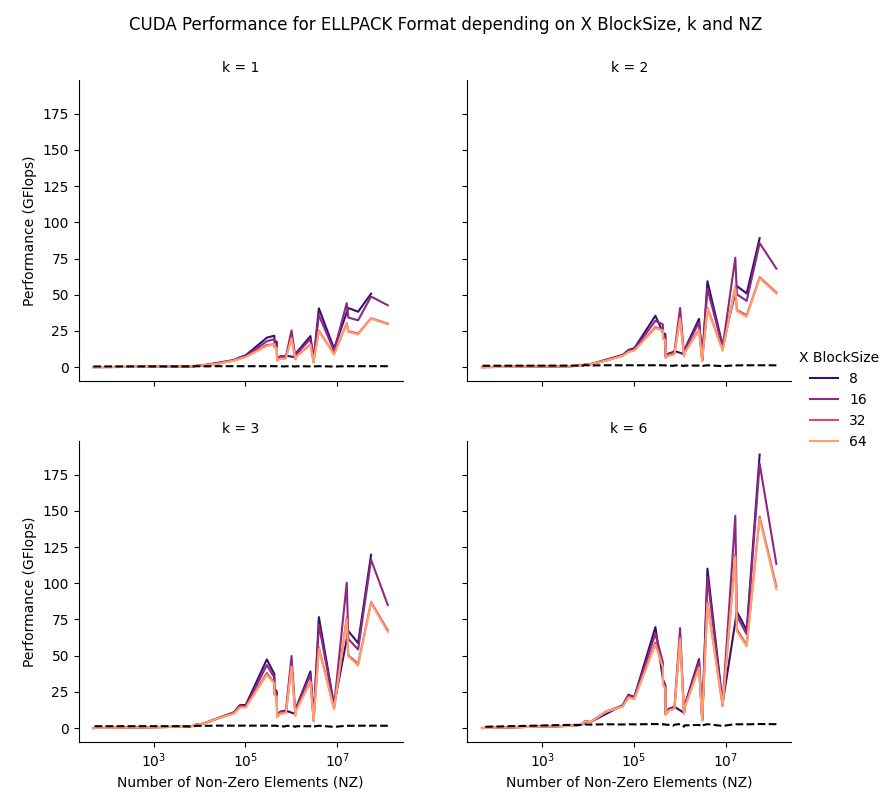
\includegraphics[width=0.75\textwidth]{../results/images/CUDA_xBlockSize_ELLPACK.png}
    \caption{CUDA Performance for ELLPACK Format depending on X BlockSize}
    \label{fig:cudaxblocksizeellpack}
\end{figure}

\begin{figure}[H]
    \centering
    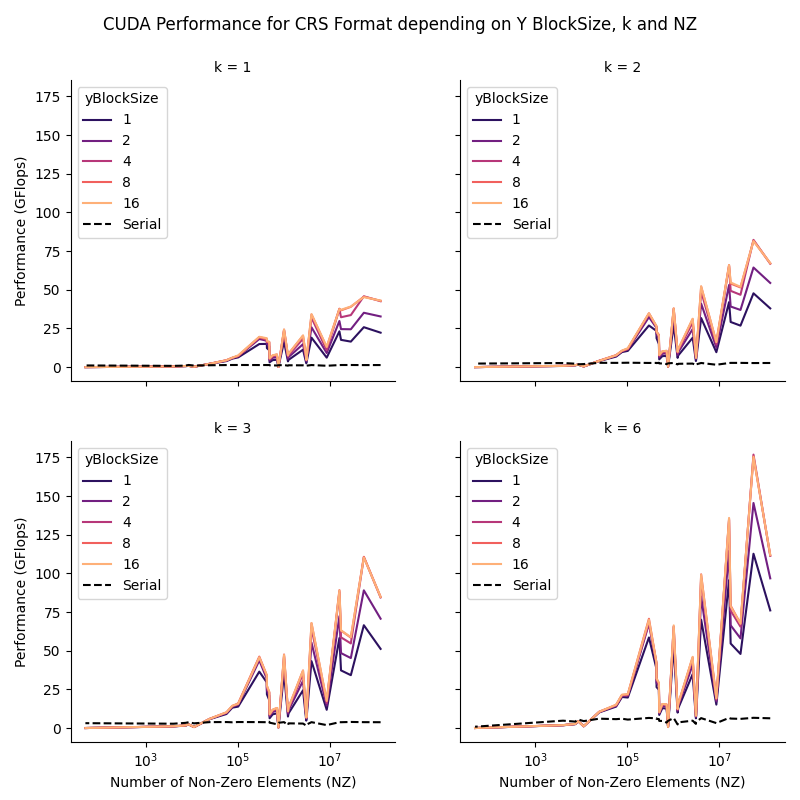
\includegraphics[width=0.75\textwidth]{../results/images/CUDA_yBlockSize_CRS.png}
    \caption{CUDA Performance for CRS Format depending on Y BlockSize}
    \label{fig:cudayblocksizecrs}
\end{figure}

\begin{figure}[H]
    \centering
    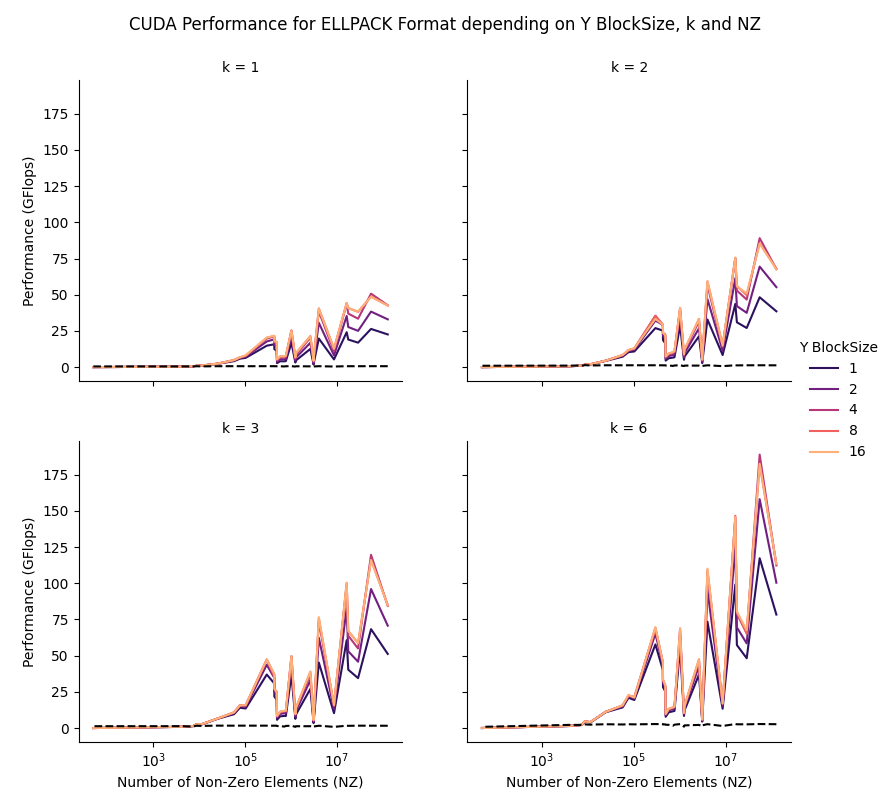
\includegraphics[width=0.75\textwidth]{../results/images/CUDA_yBlockSize_ELLPACK.png}
    \caption{CUDA Performance for ELLPACK Format depending on Y BlockSize}
    \label{fig:cudayblocksizeellpack}
\end{figure}

\newpage
\begin{figure}[H]
    \centering
    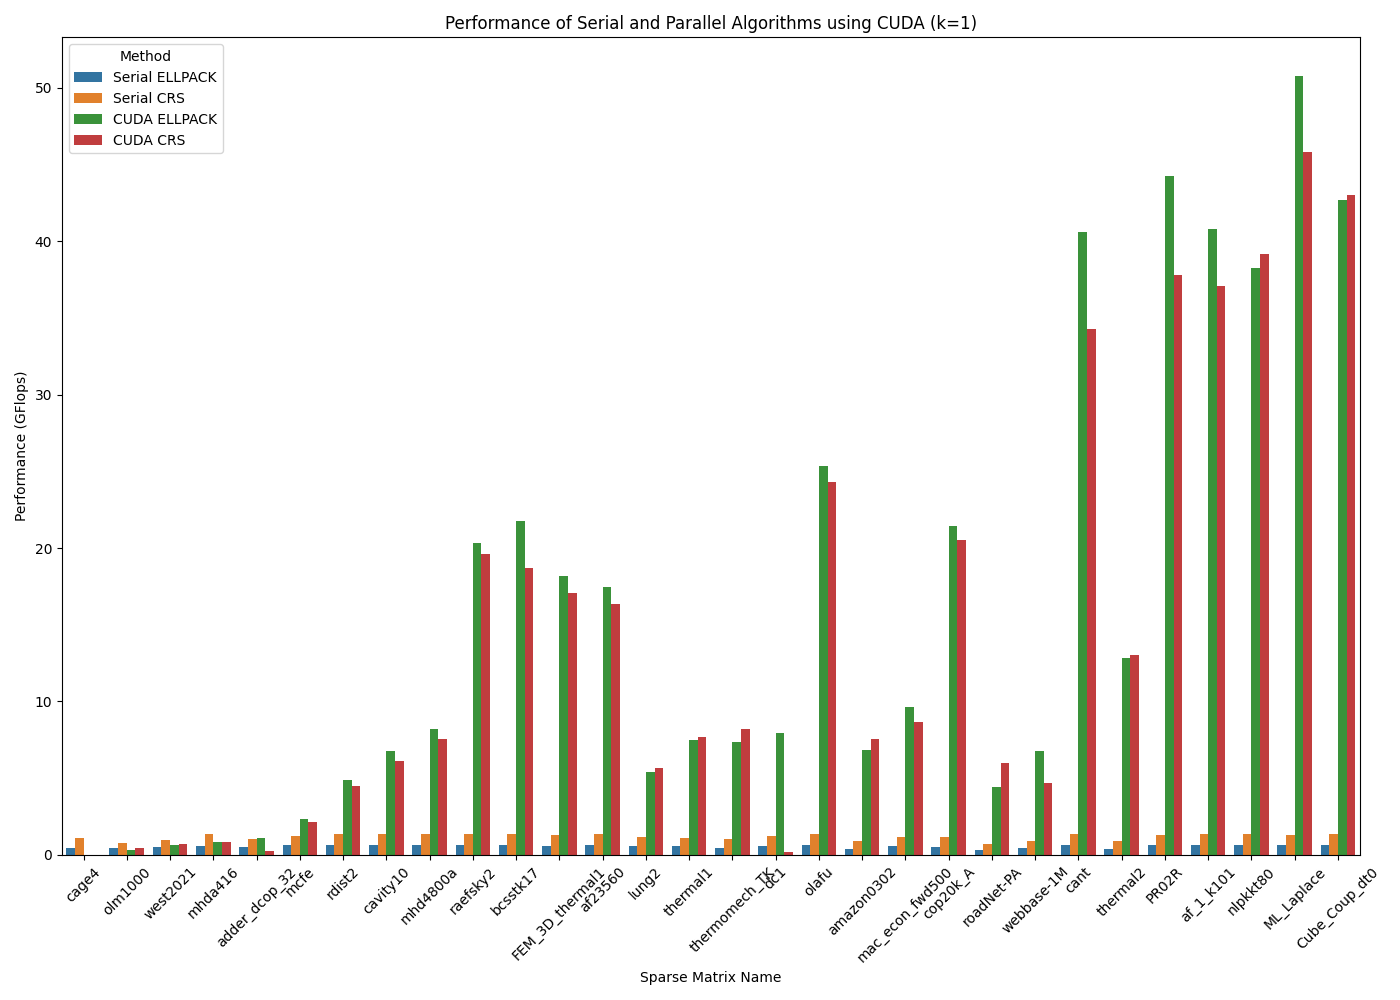
\includegraphics[width=0.9\textwidth]{../results/images/CUDA_Performance_k1.png}
    \caption{Performance of Serial and Parallel Algorithms using CUDA for $k=1$}
    \label{fig:cuda-performance-k1}
\end{figure}

\begin{figure}[H]
    \centering
    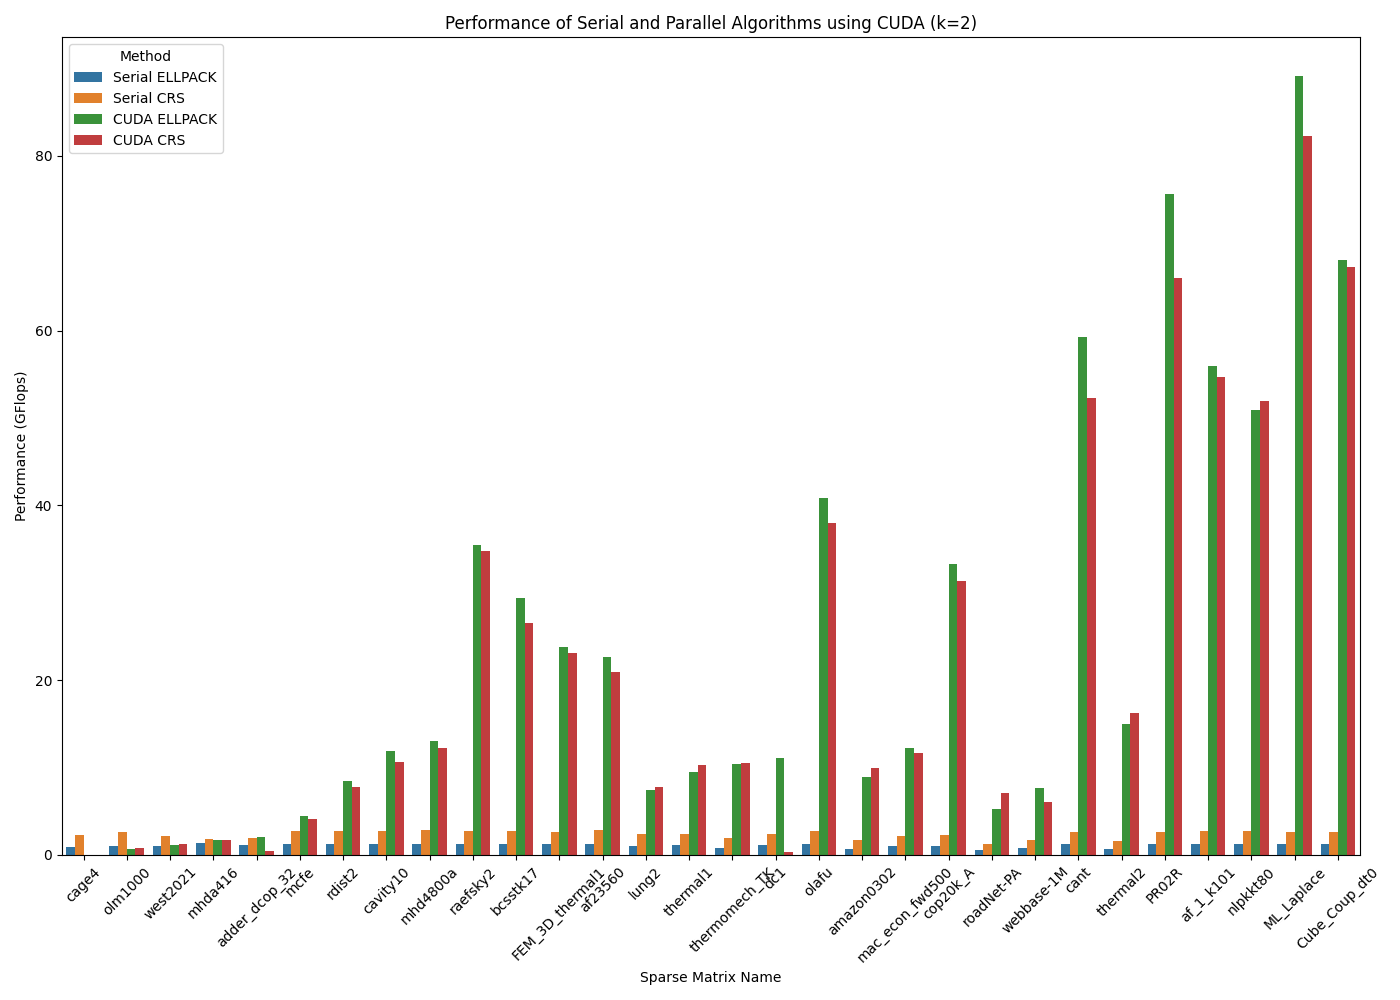
\includegraphics[width=0.9\textwidth]{../results/images/CUDA_Performance_k2.png}
    \caption{Performance of Serial and Parallel Algorithms using CUDA for $k=2$}
    \label{fig:cuda-performance-k2}
\end{figure}

\begin{figure}[H]
    \centering
    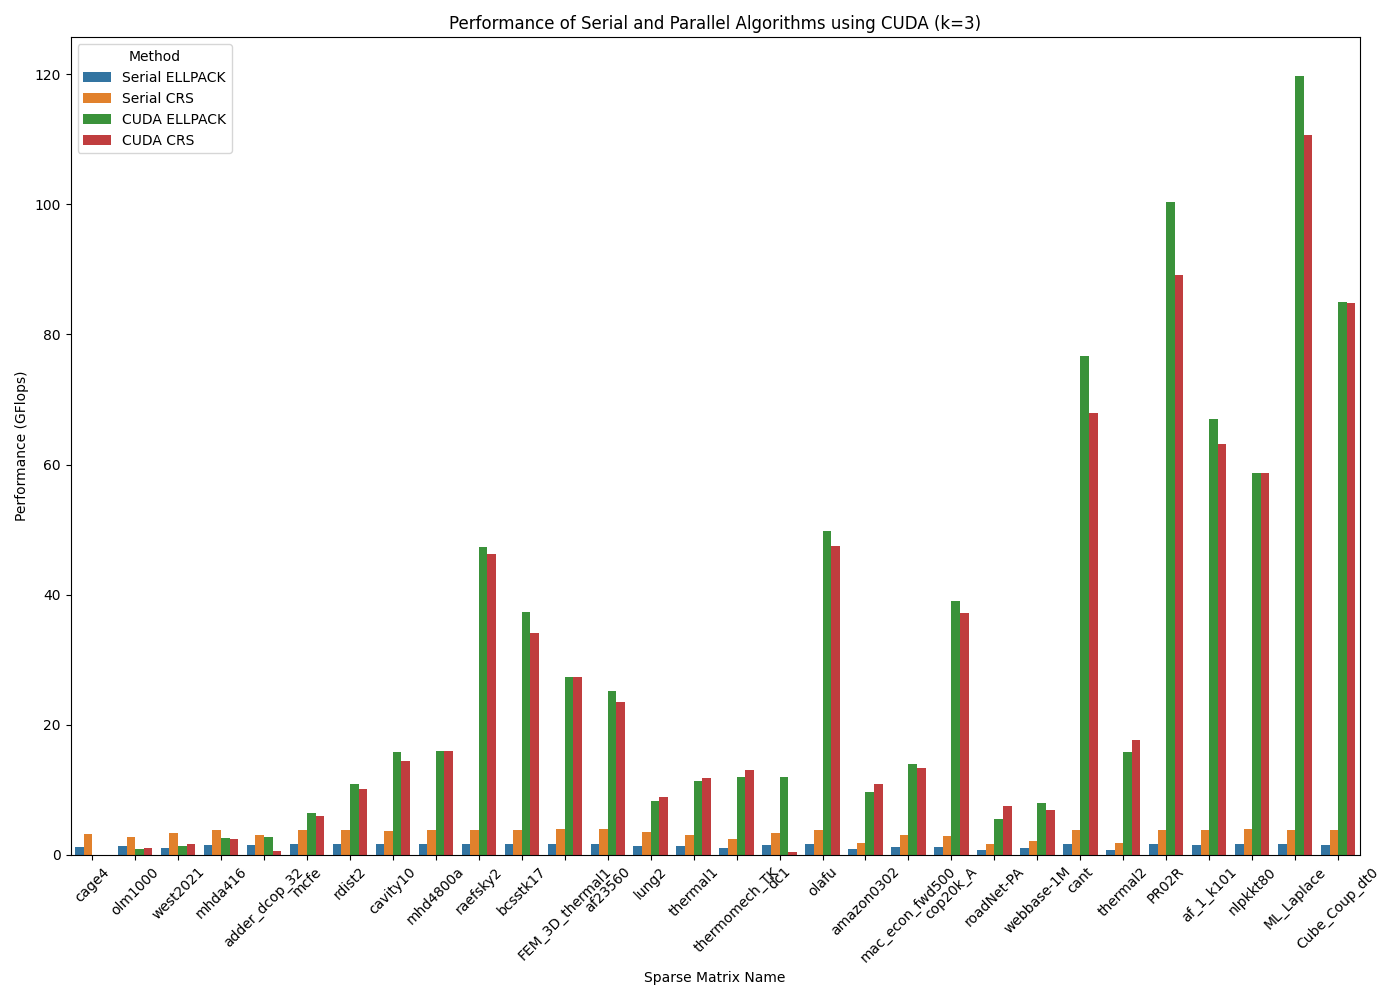
\includegraphics[width=0.9\textwidth]{../results/images/CUDA_Performance_k3.png}
    \caption{Performance of Serial and Parallel Algorithms using CUDA for $k=3$}
    \label{fig:cuda-performance-k3}
\end{figure}

\begin{figure}[H]
    \centering
    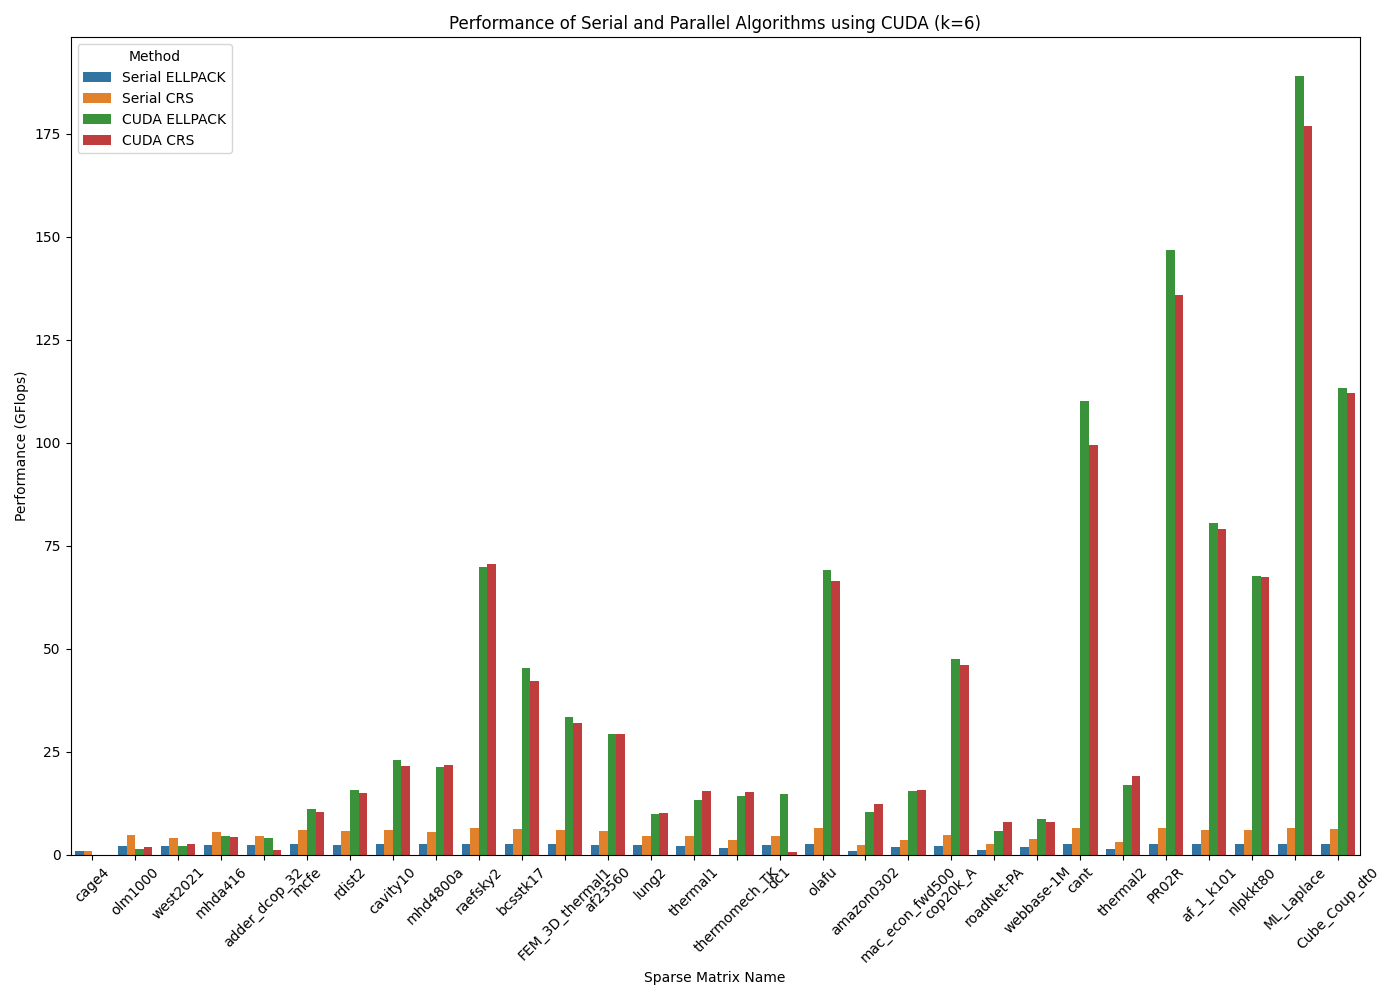
\includegraphics[width=0.9\textwidth]{../results/images/CUDA_Performance_k6.png}
    \caption{Performance of Serial and Parallel Algorithms using CUDA for $k=6$}
    \label{fig:cuda-performance-k6}
\end{figure}

\newpage
\begin{longtable}{lcccr}
    \caption{Comparaison des Performances des Algorithmes CRS et ELLPACK avec CUDA}                  \\
    \toprule
    \textbf{Matrix}   & \textbf{CRS} & \textbf{ELLPACK} & \textbf{Best Structure} & \textbf{Speedup} \\
    \midrule
    \endfirsthead
    \toprule
    \textbf{Matrix}   & \textbf{CRS} & \textbf{ELLPACK} & \textbf{Best Structure} & \textbf{Speedup} \\
    \midrule
    \endhead
    \bottomrule
    \endfoot
    amazon0302        & 12.3120      & 10.4822          & CRS                     & 5.252515         \\
    cage4             & 0.033586     & 0.031649         & CRS                     & 0.038533         \\
    lung2             & 10.2714      & 9.81548          & CRS                     & 2.216157         \\
    mac\_econ\_fwd500 & 15.6609      & 15.4014          & CRS                     & 4.250389         \\
    mhd4800a          & 21.9362      & 21.4274          & CRS                     & 4.007095         \\
    olm1000           & 1.89504      & 1.48348          & CRS                     & 0.396840         \\
    raefsky2          & 70.6624      & 69.7615          & CRS                     & 10.778230        \\
    roadNet-PA        & 8.07317      & 5.84257          & CRS                     & 2.966768         \\
    thermal1          & 15.5753      & 13.318           & CRS                     & 3.386097         \\
    thermal2          & 19.2541      & 17.0523          & CRS                     & 6.004222         \\
    thermomech\_TK    & 15.3241      & 14.2953          & CRS                     & 4.305889         \\
    west2021          & 2.66929      & 2.26954          & CRS                     & 0.637915         \\
    Cube\_Coup\_dt0   & 111.963      & 113.348          & ELLPACK                 & 17.953161        \\
    FEM\_3D\_thermal1 & 32.0555      & 33.4671          & ELLPACK                 & 5.634524         \\
    ML\_Laplace       & 176.774      & 188.886          & ELLPACK                 & 28.493590        \\
    PR02R             & 135.828      & 146.651          & ELLPACK                 & 22.294501        \\
    adder\_dcop\_32   & 1.20824      & 4.12316          & ELLPACK                 & 0.920089         \\
    af23560           & 29.2923      & 29.4083          & ELLPACK                 & 5.066518         \\
    af\_1\_k101       & 79.1365      & 80.4176          & ELLPACK                 & 13.098161        \\
    bcsstk17          & 42.2982      & 45.3715          & ELLPACK                 & 7.251562         \\
    cant              & 99.3766      & 110.127          & ELLPACK                 & 17.154513        \\
    cavity10          & 21.571       & 23.0165          & ELLPACK                 & 3.815625         \\
    cop20k\_A         & 46.062       & 47.6264          & ELLPACK                 & 9.980867         \\
    dc1               & 0.733577     & 14.7532          & ELLPACK                 & 3.147779         \\
    mcfe              & 10.5186      & 11.2408          & ELLPACK                 & 1.852130         \\
    mhda416           & 4.46372      & 4.6875           & ELLPACK                 & 0.848498         \\
    nlpkkt80          & 67.4344      & 67.5926          & ELLPACK                 & 11.394303        \\
    olafu             & 66.3819      & 69.052           & ELLPACK                 & 10.654512        \\
    rdist2            & 15.0779      & 15.7503          & ELLPACK                 & 2.733008         \\
    webbase-1M        & 8.04237      & 8.68042          & ELLPACK                 & 2.314507         \\
\end{longtable}

\newpage
\begin{figure}[H]
    \centering
    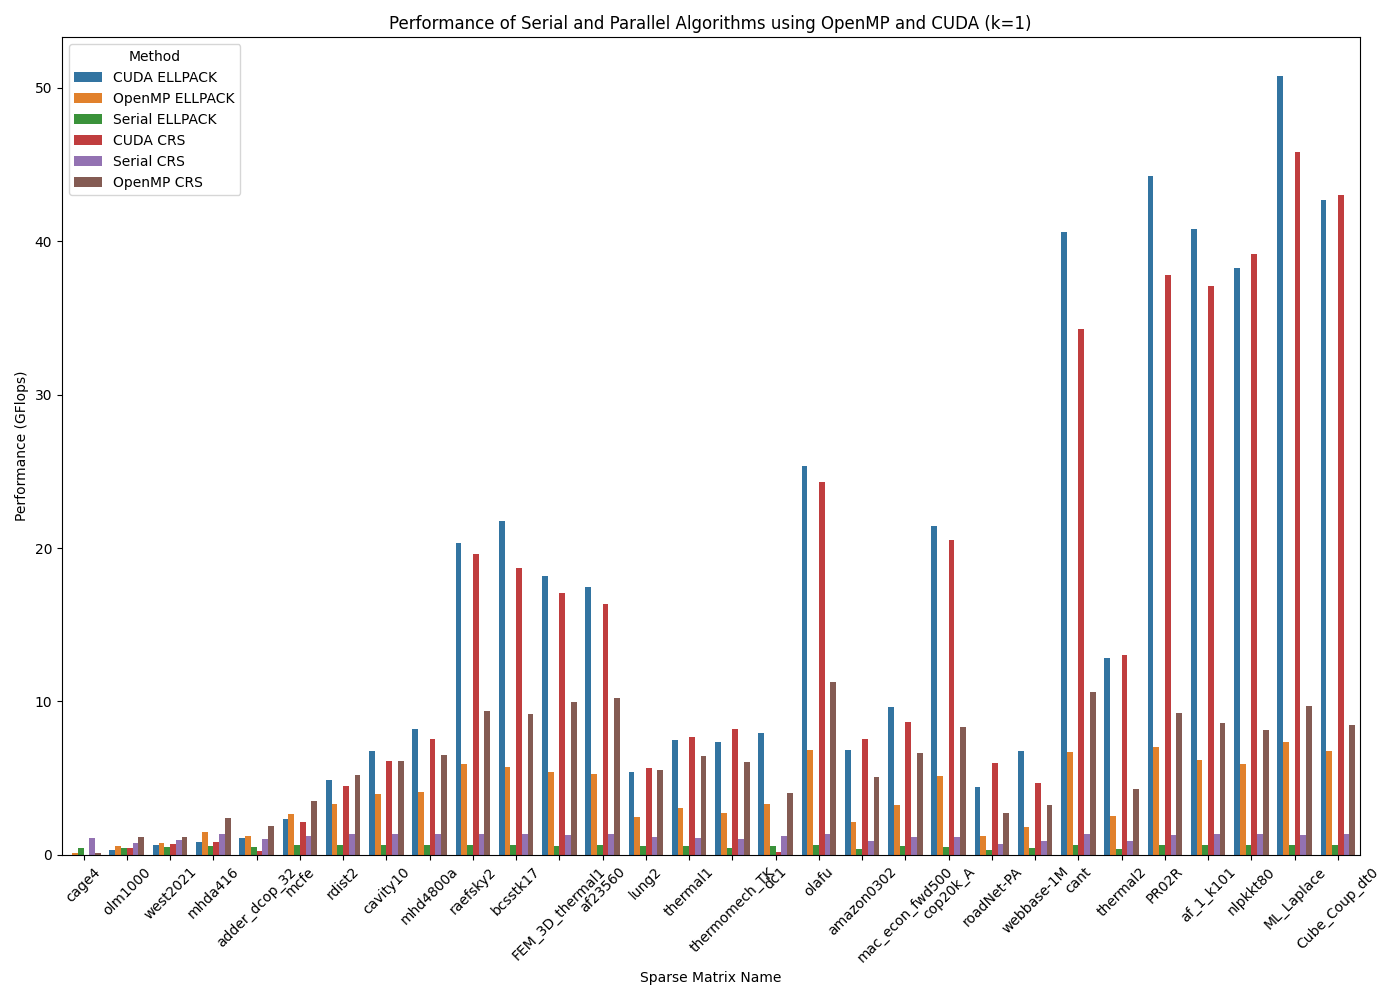
\includegraphics[width=0.9\textwidth]{../results/images/OpenMP_vs_CUDA_Performance_k1.png}
    \caption{OpenMP vs CUDA Performance for $k=1$}
    \label{fig:openmp-cuda-performance-k1}
\end{figure}

\begin{figure}[H]
    \centering
    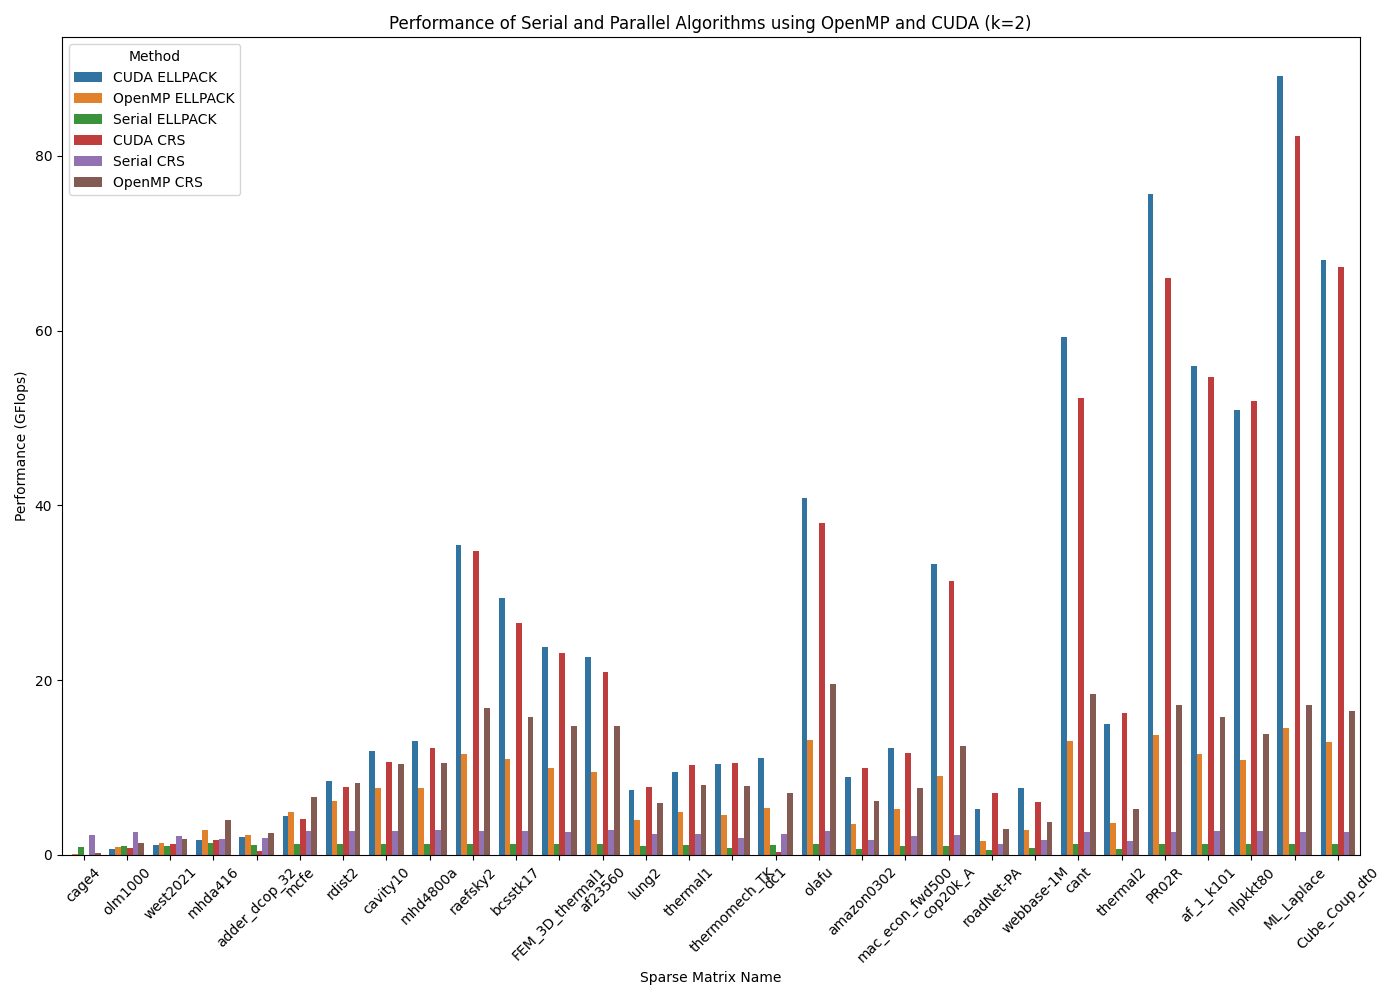
\includegraphics[width=0.9\textwidth]{../results/images/OpenMP_vs_CUDA_Performance_k2.png}
    \caption{OpenMP vs CUDA Performance for $k=2$}
    \label{fig:openmp-cuda-performance-k2}
\end{figure}

\begin{figure}[H]
    \centering
    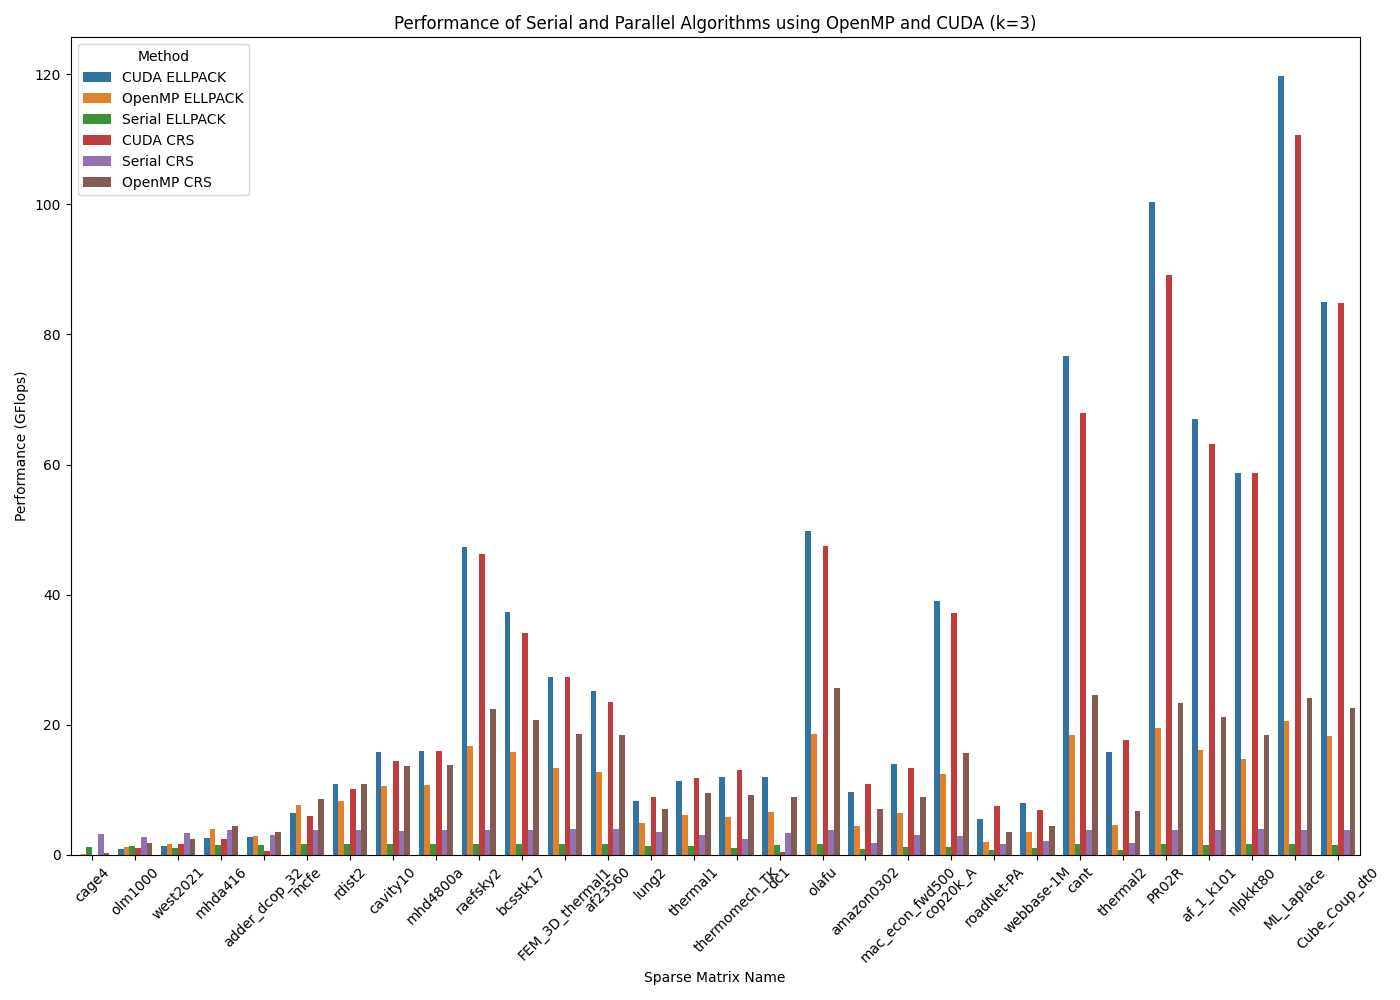
\includegraphics[width=0.9\textwidth]{../results/images/OpenMP_vs_CUDA_Performance_k3.png}
    \caption{OpenMP vs CUDA Performance for $k=3$}
    \label{fig:openmp-cuda-performance-k3}
\end{figure}

\begin{figure}[H]
    \centering
    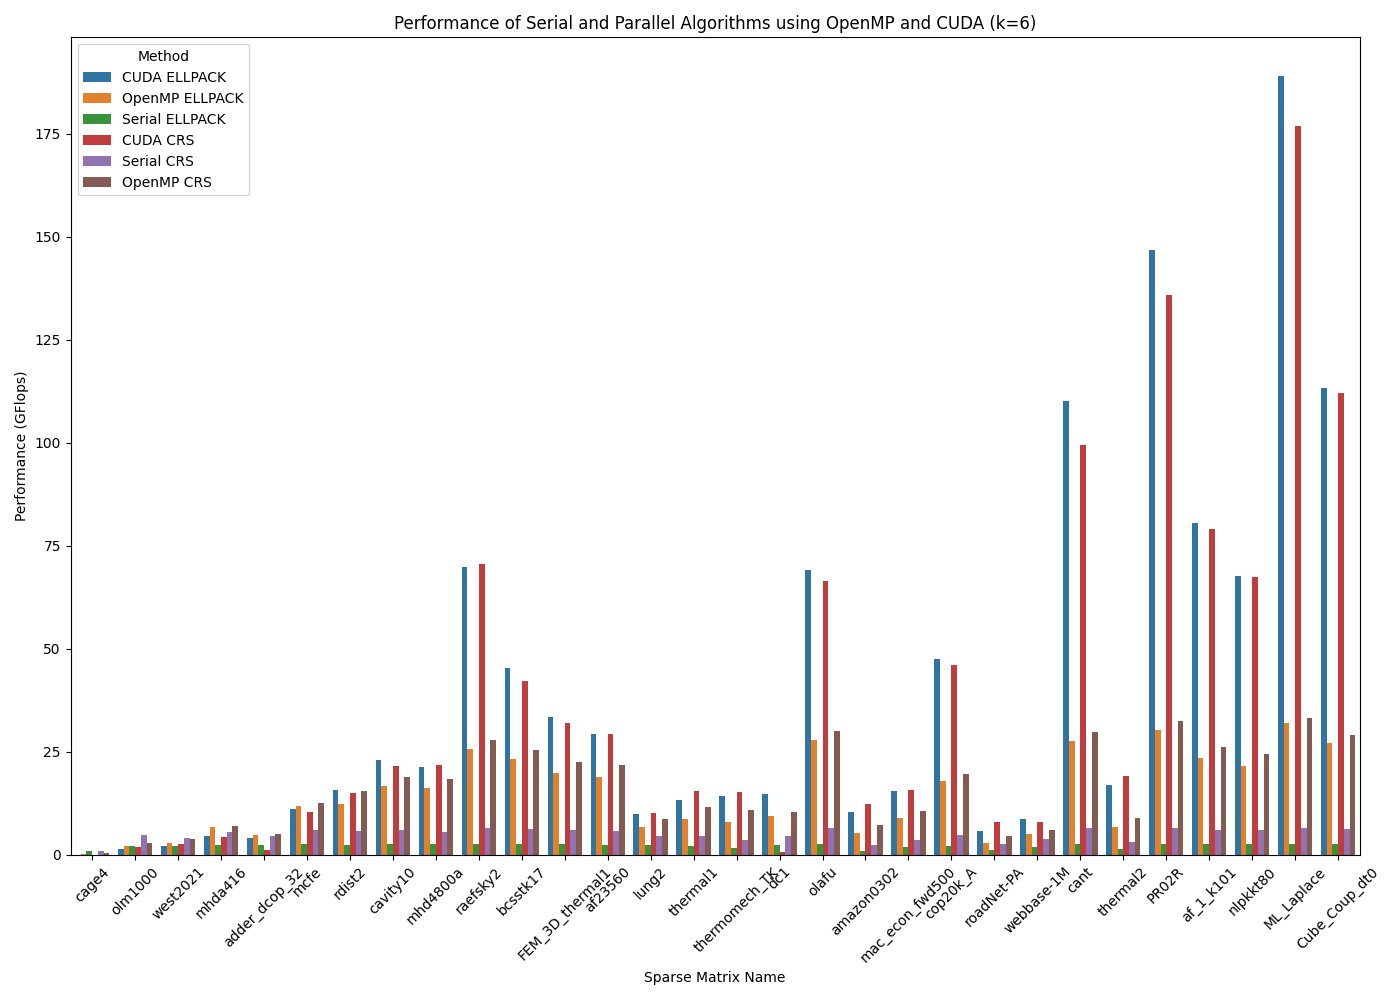
\includegraphics[width=0.9\textwidth]{../results/images/OpenMP_vs_CUDA_Performance_k6.png}
    \caption{OpenMP vs CUDA Performance for $k=6$}
    \label{fig:openmp-cuda-performance-k6}
\end{figure}

\newpage
\begin{longtable}{lccccr}
    \caption{Comparaison des Performances entre CUDA, OpenMP, et Séquentiel}                                          \\
    \toprule
    \textbf{Matrix}   & \textbf{Best Performance} & \textbf{Best Structure} & \textbf{Best Method} & \textbf{Speedup} \\
    \midrule
    \endfirsthead
    \toprule
    \textbf{Matrix}   & \textbf{Best Performance} & \textbf{Best Structure} & \textbf{Best Method} & \textbf{Speedup} \\
    \midrule
    \endhead
    \bottomrule
    \endfoot
    amazon0302        & 12.3120                   & CRS                     & CUDA                 & 5.252515         \\
    lung2             & 10.2714                   & CRS                     & CUDA                 & 2.216157         \\
    mac\_econ\_fwd500 & 15.6609                   & CRS                     & CUDA                 & 4.250389         \\
    mhd4800a          & 21.9362                   & CRS                     & CUDA                 & 4.007095         \\
    raefsky2          & 70.6624                   & CRS                     & CUDA                 & 10.778230        \\
    roadNet-PA        & 8.07317                   & CRS                     & CUDA                 & 2.966768         \\
    thermal1          & 15.5753                   & CRS                     & CUDA                 & 3.386097         \\
    thermal2          & 19.2541                   & CRS                     & CUDA                 & 6.004222         \\
    thermomech\_TK    & 15.3241                   & CRS                     & CUDA                 & 4.305889         \\
    Cube\_Coup\_dt0   & 113.348                   & ELLPACK                 & CUDA                 & 17.953161        \\
    FEM\_3D\_thermal1 & 33.4671                   & ELLPACK                 & CUDA                 & 5.634524         \\
    ML\_Laplace       & 188.886                   & ELLPACK                 & CUDA                 & 28.493590        \\
    PR02R             & 146.651                   & ELLPACK                 & CUDA                 & 22.294501        \\
    af23560           & 29.4083                   & ELLPACK                 & CUDA                 & 5.066518         \\
    af\_1\_k101       & 80.4176                   & ELLPACK                 & CUDA                 & 13.098161        \\
    bcsstk17          & 45.3715                   & ELLPACK                 & CUDA                 & 7.251562         \\
    cant              & 110.127                   & ELLPACK                 & CUDA                 & 17.154513        \\
    cavity10          & 23.0165                   & ELLPACK                 & CUDA                 & 3.815625         \\
    cop20k\_A         & 47.6264                   & ELLPACK                 & CUDA                 & 9.980867         \\
    dc1               & 14.7532                   & ELLPACK                 & CUDA                 & 3.147779         \\
    nlpkkt80          & 67.5926                   & ELLPACK                 & CUDA                 & 11.394303        \\
    olafu             & 69.0520                   & ELLPACK                 & CUDA                 & 10.654512        \\
    rdist2            & 15.7503                   & ELLPACK                 & CUDA                 & 2.733008         \\
    webbase-1M        & 8.68042                   & ELLPACK                 & CUDA                 & 2.314507         \\
    adder\_dcop\_32   & 5.12204                   & CRS                     & OpenMP               & 1.142991         \\
    mcfe              & 12.6097                   & CRS                     & OpenMP               & 2.077682         \\
    mhda416           & 7.06099                   & CRS                     & OpenMP               & 1.278130         \\
    cage4             & 0.871628                  & CRS                     & Serial               & 1.000000         \\
    olm1000           & 4.77532                   & CRS                     & Serial               & 1.000000         \\
    west2021          & 4.1844                    & CRS                     & Serial               & 1.000000         \\
\end{longtable}

\chapter{Conclusion}

In conclusion, this report has meticulously analysed various parallelization
strategies for fat matrix vector multiplication, based on the MPI and PETSc
frameworks, and through extensive experimentation and comparison, highlights
the importance of choosing an appropriate parallelization approach based on
matrix characteristics and computational resources. The results highlight the
trade-offs between computational and communication overheads, emphasising the
need for a balanced distribution of workloads to maximise efficiency. As
expected the PETSc library outperforms the custom implementations in terms of
execution time but not in terms of performance, as the matrices stay
distributed even after the multiplication. The custom implementations are more
efficient to reconstruct the final result from the gathered vector. In
addition, the discussion of the environmental impact of HPC practices, with a
nod to sustainable computing, reflects a broader perspective on the
implications of computational research. Future directions could explore
adaptive parallelization techniques, further optimizing specific models and
matrix sizes, possibly integrating AI for dynamic algorithm selection based on
real-time performance metrics. This study not only contributes to the field of
HPC by providing insight into efficient algorithmic implementations, but also
paves the way for more energy-efficient HPC systems, in line with global
sustainable development goals.

\bibliographystyle{CranfieldNumbered}
\bibliography{CUCitations}

%TC:ignore 
\appendix
\chapter{Documentation}

\begin{subappendices}
    \section{Project tree}
    \begin{lstlisting}[breaklines=true, basicstyle=\small]
    Source Code/
        scripts/
            batch_test.sh
            get_csv_all.sh
            get_csv_debug.sh
            get_csv_specific.sh
            mpi.sub
        MatrixDefinitions.h
        SparseMatrixFatVectorMultiply.h
        SparseMatrixFatVectorMultiply.cpp
        SparseMatrixFatVectorMultiplyRowWise.h
        SparseMatrixFatVectorMultiplyRowWise.cpp
        SparseMatrixFatVectorMultiplyColumnWise.h
        SparseMatrixFatVectorMultiplyColumnWise.cpp
        SparseMatrixFatVectorMultiplyNonZeroElement.h
        SparseMatrixFatVectorMultiplyNonZeroElement.cpp
        utils.h
        utils.cpp
        main.cpp
    results/
        fat_vector_dim/
            <sparse_matrix>_<k>_<metric>.png
        matrix_dim/
            <sparse_matrix>_<k>_<metric>.png
    \end{lstlisting}

    \section{Getting Started}
    To run the program, follow these steps:
    \begin{enumerate}
        \itemindent=17.87pt
        \item Install the required libraries:
              \href{https://docs.open-mpi.org/en/main/installing-open-mpi/quickstart.html}{mpi}
              \& \href{https://petsc.org/release/install/}{petsc}
        \item Compile the main program using the following command:
              \begin{lstlisting}[style=bashstyle]
                mmpicxx -o <executable_name> -I${PETSC_DIR}/include -I${PETSC_DIR}/${PETSC_ARCH}/include -L${PETSC_DIR}/${PETSC_ARCH}/lib -lpetsc SparseMatrixFatVectorMultiply.cpp  main_verify.cpp utils.cpp SparseMatrixFatVectorMultiplyColumnWise.cpp SparseMatrixFatVectorMultiplyNonZeroElement.cpp SparseMatrixFatVectorMultiplyRowWise.cpp
            \end{lstlisting}
        \item Run the program using the following command:
              \begin{lstlisting}[style=bashstyle]
                mpirun -np <number_of_processes> <executable_name> <k> <sparse_matrix_file_pathw>
            \end{lstlisting}
    \end{enumerate}

    \section{Methods Overview}
    \subsection{Utils.h}
    \subsubsection{ConvertPETScMatToFatVector}

    \textbf{Description:} Converts a PETSc matrix to a FatVector stucture.\\

    \textbf{Parameters:}
    \begin{itemize}
        \item \texttt{Mat C} - PETSc matrix to be converted.
    \end{itemize}

    \textbf{Returns:} \texttt{FatVector} - Fat vector representation of the PETSc matrix.

    \subsubsection{areMatricesEqual}
    \textbf{Description:} Compares two matrices for equality within a specified tolerance.\\

    \textbf{Parameters:}
    \begin{itemize}
        \item \texttt{FatVector \&mat1} - First matrix.
        \item \texttt{FatVector \&mat2} - Second matrix.
        \item \texttt{double tolerance} - Tolerance for comparison.
    \end{itemize}

    \textbf{Returns:} \texttt{bool} - True if matrices are equal within the tolerance, false otherwise.

    \subsubsection{readMatrixMarketFile}
    \textbf{Description:} Reads a matrix from a Matrix Market file into a sparse matrix format.\\

    \textbf{Parameters:}
    \begin{itemize}
        \item \texttt{std::string \&filename} - Name of the Matrix Market file.
    \end{itemize}

    \textbf{Returns:} \texttt{SparseMatrix} - Sparse matrix read from the file.

    \subsubsection{generateLargeFatVector}
    \textbf{Description:} Generates a random Fat Vector with specified dimensions.\\

    \textbf{Parameters:}
    \begin{itemize}
        \item \texttt{int n} - Number of rows.
        \item \texttt{int k} - Number of columns.
    \end{itemize}

    \textbf{Returns:} \texttt{FatVector} - Generated fat vector.

    \subsubsection{serialize and deserialize}
    \textbf{Description:} Serializes and deserializes a FatVector to and from a flat array, respectively.\\

    \textbf{Parameters for serialize:}
    \begin{itemize}
        \item \texttt{FatVector \&fatVec} - fat vector to serialize.
    \end{itemize}

    \textbf{Returns:} \texttt{std::vector<double>} - Flat array containing the serialized data.\\

    \textbf{Parameters for deserialize:}
    \begin{itemize}
        \item \texttt{std::vector<double> \&flat} - Flat array to deserialize.
        \item \texttt{int rows} - Number of rows in the fat vector.
        \item \texttt{int cols} - Number of columns in the fat vector.
    \end{itemize}

    \textbf{Returns:} \texttt{FatVector} - Deserialized fat vector.

    \subsection{SparseMatrixFatVectorMultiply.h}
    \subsubsection{sparseMatrixFatVectorMultiply}
    \textbf{Description:} Executes the multiplication using a sequential algorithm.\\

    \textbf{Parameters:}
    \begin{itemize}
        \item \texttt{SparseMatrix \&sparseMatrix} - The sparse matrix.
        \item \texttt{FatVector \&fatVector} - The Fat Vector.
        \item \texttt{int vecCols} - Number of columns in the Fat Vector.
    \end{itemize}

    \textbf{Returns:} \texttt{FatVector} - Result of the multiplication.

    \subsection{SparseMatrixFatVectorMultiplyRowWise.h}
    \subsubsection{sparseMatrixFatVectorMultiplyRowWise}
    \textbf{Description:} Multiplies a sparse matrix with a Fat Vector using row-wise distribution.\\

    \textbf{Parameters:}
    \begin{itemize}
        \item \texttt{SparseMatrix \&sparseMatrix} - The sparse matrix.
        \item \texttt{FatVector \&fatVector} - The Fat Vector.
        \item \texttt{int vecCols} - Number of columns in the Fat Vector.
    \end{itemize}

    \textbf{Returns:} \texttt{FatVector} - Result of the multiplication.

    \subsection{SparseMatrixFatVectorMultiplyColumnWise.h}
    \subsubsection{sparseMatrixFatVectorMultiplyColumnWise}
    \textbf{Description:} Executes the multiplication using column-wise parallel algorithm.\\

    \textbf{Parameters:}
    \begin{itemize}
        \item \texttt{SparseMatrix \&sparseMatrix} - The sparse matrix.
        \item \texttt{FatVector \&fatVector} - The Fat Vector.
        \item \texttt{int vecCols} - Number of columns in the Fat Vector.
    \end{itemize}

    \textbf{Returns:} \texttt{FatVector} - Result of the multiplication.

    \subsection{SparseMatrixFatVectorMultiplyNonZeroElement.h}
    \subsubsection{sparseMatrixFatVectorMultiplyNonZeroElement}
    \textbf{Description:} Executes the multiplication using non-zero element parallel algorithm.\\

    \textbf{Parameters:}
    \begin{itemize}
        \item \texttt{SparseMatrix \&sparseMatrix} - The sparse matrix.
        \item \texttt{FatVector \&fatVector} - The Fat Vector.
        \item \texttt{int vecCols} - Number of columns in the Fat Vector.
    \end{itemize}

    \textbf{Returns:} \texttt{FatVector} - Result of the multiplication.

\end{subappendices}

\chapter{Source Codes}
\begin{subappendices}
    \section{Data Structures}\label{appendix:data-structures}
    Data stuctures of the sparse matrix and fat vector.

\end{subappendices}
%TC:endignore 

\end{document}

